\documentclass[a4paper,12pt]{article}
\usepackage[margin=2cm]{geometry}

% Pacchetti utili di base
\usepackage[utf8]{inputenc}   % codifica dei caratteri
\usepackage[T1]{fontenc}      % font encoding
\usepackage[italian]{babel}   % lingua italiana
\usepackage{graphicx}         % immagini
\usepackage{hyperref}         % link cliccabili
\usepackage{amsmath}          % align center
\usepackage{listings}         %codice programmazione
\usepackage{xcolor}           % per colori opzionali del codice
\usepackage{float}

\lstset{escapeinside={<@}{@>}}
% Definizione linguaggio MIPS per listings
\lstdefinelanguage{MIPS}{
  morekeywords={lw,sw,add,sub,addi,li,la,j,jr,jal,move,beq,bne,slt},
  sensitive=true,
  morecomment=[l]{\#},      % commento con #
  morestring=[b]"           % stringhe tra doppi apici
}

% Informazioni sul documento
\title{Sistemi Operativi}
\author{Nicolò Giuliani}
\date{}


\begin{document}
\maketitle
\tableofcontents   % <-- genera automaticamente la pagina dell'indice
\newpage 

\section{Concorrenza}
\subsection{Introduzione alla concorrenza}
Un sistema operativo consiste in un gran numero di attività che vengono eseguite più o meno contemporaneamente dal processore e dai dispositivi presenti in un elaboratore. Ovviamente bisogna far coesistere le diverse attività attraverso il \texttt{modello concorrente} e il concetto di \texttt{processo}. \\
Cosa è questo processo? E' una singola attività di un programma che il processore deve eseguire, questo vuol dire che processo $\neq$ programma. Il programma è statico (insieme di istruzioni) mentre il processo è \textit{dinamico}, ovvero l'attività di esecuzione di un programma. Attraverso l'assioma di \textbf{finite process} determiniamo che un processo viene eseguito sempre ad una velocità sconosciuta finita, mai nulla.
\paragraph{Come descriviamo un processo?} 
\begin{itemize}
  \item Immagine della memoria: \\
  - la memoria assegnata al singolo processo e le strutture dati del S.O. associate al processo (es. file aperti).
  \item Immagine del processore: \\
  - Registri della CPU
  \item Stato di avanzamento: \\
  - Running: in esecuzione \\
  - Waiting: in attesa di evento esterno / non può essere esguito \\ 
  - Ready: può essere eseguito ma la CPU è occupata
\end{itemize}
\begin{figure}[h] % [h] = qui (here)
    \centering
    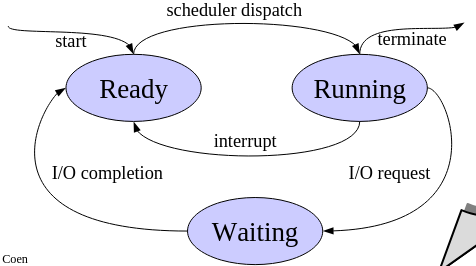
\includegraphics[width=0.5\textwidth]{img/status_processo.png}
\end{figure}
\paragraph{Cosa è la concorrenza?\\} 
Gestione dei processi \textit{multipli} per la comunicazione e sincronizzazione:
\begin{itemize}
  \item Multiprogramming: più processi su un singolo processore (parallelismo apparente) \\
  - i processi sono "alternati nel tempo", quindi 1 sola operazione per istante. Si definisce \textbf{interliving}
  \item Multiprocessing: più processi su più processori (parallelismo reale) \\
  - i processi sono "alternati nello spazio" ovvero eseguiti simultaneamente su processori diversi. Si definisce \textbf{overlapping}
  \item Distributed processing: più processi su più computer separati (parallelismo reale)
\end{itemize}
Definiamo in \textit{esecuzione concorrente} due programmi eseguiti in parallelo (apparente/reale). Sia in caso di interliving che per l'overlapping abbiamo gli stessi problemi comuni: predire la velocità dei processi! \\
Esempio: \\
\begin{minipage}{0.48\textwidth}
\begin{lstlisting}[language=C]
void modifica(int valore){
  totale += valore;
}
\end{lstlisting}
\end{minipage}
\hfill
\begin{minipage}{0.48\textwidth}
\begin{lstlisting}[language={[x86masm]Assembler}]
section .data
.text
modifica:
    lw $t0, totale
    add $t0, $t0, $a0
    sw $t0, totale
    jr $ra
\end{lstlisting}
\end{minipage}
Ipotizziamo che esecuiamo $P_1$ con $modifica(+10)$ e $P_2$ con $modifica(-10)$ in esecuzione corrente con la variabile $totale$ in comune. Analizziamo l'assembly:
\begin{lstlisting}[language=MIPS]
P1 lw $t0, totale             totale=100, $t0=100, $a0=10
P1 add $t0, $t0, $a0          totale=100, $t0=110, $a0=10
P1 sw $t0, totale             totale=110, $t0=110, $a0=10

S.O. interrupt
S.O. salvataggio registri P1
S.O. ripristino registri P2   totale=110, $t0=?, $a0=-10

P2 lw $t0, totale             totale=110, $t0=110, $a0=-10
P2 add $t0, $t0, $a0          totale=110, $t0=100, $a0=-10
P2 sw $t0, totale             totale=100, $t0=100, $a0=-10
\end{lstlisting}
Quindi i due processi non possono essere eseguti contemporaneamente da due processori distinti perchè la variabile $totale$ non può essere accessa simultaneamente. 
\vspace{1em}\\Definiamo \textbf{race condition} quando il risultato corretto dipenda dalla temporizzazione dei processi. Per questo esiste lo \textbf{scheduler} ovvero il componente del SO che decide il processo da eseguire in determininato momento.
\subsection{Interazioni tra processi}
\begin{itemize}
  \item Processi indirettamente a conoscienza uno dell'altro (memoria pubblica)\\
  - convididono risorse (buffer), vanno sincronizzati
  \item Processi direttamente a conoscienza uno dell'altro (memoria privata)\\
  - la comunicazione viene in base all'id, spesso diretta via messaggi 
\end{itemize}
Una \textbf{proprietà} di un programma è un attributo che rimane sempre vero per ogni esecuzione.
\begin{itemize}
  \item Safety: il programma avanza finchè è tutto ok \\
  - i processi non devono interferire tra loro nell'accesso della memoria. La sincronizzazione garantisce la proprietà.
  \item Liveness: il programma è vitale, non si ferma mai. Ha come proprietà la terminazione. \\
  - i mezzi di sincronizzazione non devono prevenire l'avanzamento del programma (no attese infinite)
\end{itemize}
Definiamo l'accesso ad una risorsa \textbf{mutualmente esclusivo} se per ogni istante solo un processo può accedervi, questo può portare ad un blocco permanente di un programma. Il \textit{deadlock} ovvero una situzione di stallo dove un processo aspetta un altro creando un attesa a cerchio infinito con mutua esclusione, hold and wait e no uscita forzata, crea una attesa infinita; la sua mancanza è una proprietà si safety.
\begin{figure}[h] % [h] = qui (here)
    \centering
    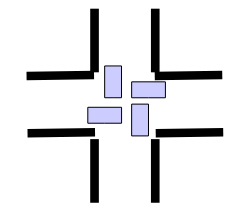
\includegraphics[width=0.3\textwidth]{img/deadlock.png}
\end{figure} \\
Quando due processi possono interferire? \\
Le \textbf{Azioni atomiche} sono operazioni che non possono essere interrotte o divise durante la loro esecuzione. Nel parallelismo reale si garantisce che l'azione non interferisca con altri processi durante la sua esecuzione. Nel caso di parallelismo apparante l'avvicendamento fra i processi avviene prima o dopo l'azione, che quindi non può interferire.
\begin{lstlisting}[language={[x86masm]Assembler}]
lw $t0, ($a0)
add $t0, $t0, $a1
sw $t0, ($a0)
\end{lstlisting}
\begin{itemize}
  \item le singole istruzioni in linguaggio macchina sono atomiche
  \item le singole istruzioni in assembly possono non essere atomiche (ci sono psuedoistruzioni)
\end{itemize}
\subsection{Sezioni critiche}
Se le sequenze di istruzioni non vengono eseguite in modo atomico, come possiamo garantire la non-interferenza? \\
Dobbiamo trovare il modo di specificare che certe parti dei programmi sono "speciali", ovvero devono essere eseguite in modo atomico (senza interruzioni). \\
Definiamo la parte di un programma che utilizza una o più risorse condivise viene detta \underline{sezione critica} (critical section, o CS) \\
\begin{minipage}{0.48\textwidth}
\begin{lstlisting}[language=C]
process P1
  a1 = read();
  <@\underline{totale = totale + a1;}@>
}
\end{lstlisting}
\end{minipage}
\hfill
\begin{minipage}{0.48\textwidth}
\begin{lstlisting}[language=C]
process P2 {
  a2 = read();
  <@\underline{totale = totale + a2;}@>
}
\end{lstlisting}
\end{minipage}
Vogliamo garantire che le sezioni critiche siano eseguite in modo mutualmente esclusivo (atomico), dobbiamo evitare il deadlock e starvation. \\
\begin{minipage}{0.48\textwidth}
\begin{lstlisting}[language=C]
Process P
  val = rand();
  a = a + val;
  b = b + val
Process Q
  val = rand();
  a = a * val;
  b = b * val;
\end{lstlisting}
\end{minipage}
\hfill 
\begin{minipage}{0.48\textwidth}
\begin{lstlisting}[language=C]
Process P
  val = rand();
  [enter cs]
  a = a + val;
  b = b + val
  [exit cs]
Process Q
  val = rand();
  [enter cs]
  a = a * val;
  b = b * val;
  [exit cs]
\end{lstlisting}
\end{minipage}
Indichiamo al S.O. cosa può essere eseguito in parallelo e cosa no (in modo atomico).
\vspace{2em} \\
Ora ragioniamo sul seguente problema:
\begin{lstlisting}[language=C]
process Pi { /* i=1...N */
  while (true) {
    [enter cs]
    critical section
    [exit cs]
    non-critical section
  }
}
\end{lstlisting}
dobbiamo avere le seguenti proprietà:
\begin{itemize}
  \item Mutua esclusione: solo un processo alla volta deve essere all'interno della CS, fra tutti quelli che hanno una CS per la stessa risorsa condivisa
  \item Assenza di deadlock: uno scenario in cui tutti i processi restano bloccati definitivamente non è ammissibile
  \item Assenza di delay non necessari: un processo fuori dalla CS non deve ritardare l'ingresso della CS da parte di un altro processo
  \item Eventual entry (assenza di starvation): ogni processo che lo richiede, prima o poi entra nella CS
\end{itemize}
\vspace{15em}
- Algoritmo di Peterson: \\
\begin{lstlisting}[language=C]
shared boolean needp = false;
shared boolean needq = false;
shared int turn;
\end{lstlisting}
\begin{minipage}{0.48\textwidth}
\begin{lstlisting}[language=C]
process P {
  while (true) {
    /* entry protocol */
    needp = true;
    turn = Q;
    while (needq && turn != P) ; 
      /* do nothing */
    critical section
    needp = false;
    non-critical section
  }
}
\end{lstlisting}
\end{minipage}
\hfill 
\begin{minipage}{0.48\textwidth}
\begin{lstlisting}[language=C]
process Q {
  while (true) {
    /* entry protocol */
    needq = true;
    turn = P;
    while (needp && turn != Q) ; 
      /* do nothing */
    critical section
    needq = false;
    non-critical section
  }
}
\end{lstlisting}
\end{minipage}
Vediamo la versione per $n$ processi
\begin{lstlisting}[language=C]
shared int[] stage = new int[N]; /* 0-initialized */
shared int[] last = new int[N]; /* 0-initialized */
process Pi { /* i = 0...N-1 */
  while (true) {
    /* Entry protocol */
    for (int j=0; j < N; j++) {
      stage[i] = j; last[j] = i;
      for (int k=0; k < N; k++) {
        if (i != k)
          while (stage[k] >= stage[i] && last[j] == i)
            ;
        }
    }
    critical section
    stage[i] = 0;
    non-critical section
  }
}
\end{lstlisting}
\vspace{15em}
A livello teorico, è possibile creare istruzioni hardware speciali per semplificare la realizzazione delle sezioni critiche.  
Tali istruzioni eseguono due azioni in modo atomico, e vengono spesso utilizzate per implementare meccanismi di \textit{spinlock}.

\begin{align*}
  TS(x, y) := \langle y = x;\; x = 1 \rangle
\end{align*}

Ciò significa che, con l'operazione di \textit{Test} (controlla/legge il valore) e \textit{Set} (imposta/scrive), si legge se la risorsa condivisa $x$ è libera ($0$) o occupata ($1$), e si assegna alla variabile locale $y$ il valore precedente di $x$. L'intera operazione avviene in modo atomico.
\begin{lstlisting}[language=C]
shared int lock = 0;   // 0 = libero, 1 = occupato

process P {
    int vp;
    while (true) {
        do {
            TS(lock, vp);     // vp = lock; lock = 1 (atomico)
        } while (vp);         // se vp = 1 -> lock occupato, riprova

        critical_section();   // sezione critica (solo uno per volta)
        lock = 0;             // rilascio del lock
        non_critical_section();
    }
}

process Q {
    int vp;
    while (true) {
        do {
            TS(lock, vp);
        } while (vp);

        critical_section();
        lock = 0;
        non_critical_section();
    }
}
\end{lstlisting}
\vspace{20em}
\subsection{Semafori}
Si tratta di un paradigma per la sincronizzazione (così come i semafori stradali sincronizzano l'occupazione di un incrocio). Vediamo ora il principio alla base: due o più processi possono cooperare attraverso semplici segnali, in modo tale che un processo possa essere bloccato in specifici punti del suo programma finché non riceve un segnale da un altro processo.
\begin{lstlisting}[language=C]
Semaphore s = new Semaphore(1);
process P {
  while (true) {
    s.P();
    critical section
    s.V();
    non-critical section
  }
}
\end{lstlisting}
Analizziamo:
\begin{itemize}
  \item ogni semaforo è una variabile intera, inizializzato a valore \textbf{non negativo}
  \item P (atomico): attende che il semaforo sia \textit{positivo}, decrementa il semaforo
  \item V (atomico): incrementa il semaforo
\end{itemize}
\begin{minipage}{0.48\textwidth}
\begin{lstlisting}[language=C]
class Semaphore {
  semaphore(int v);
  void P(void);
  void V(void);
}
\end{lstlisting}
\end{minipage}
\begin{minipage}{0.48\textwidth}
\begin{itemize}
  \item $n_p$ è il numero di operazioni di $P$
  \item $n_v$ è il numero di operazioni di $V$
  \item $init$ è il valore iniziale del semaforo
\end{itemize}
Il valore del semafoto: $n_v + init - n_p$, quindi $n_P  \leq n_v + init$
\end{minipage} \\
\vspace{3em} \\
\textbf{Semafori – Implementazione nei sistemi operativi\\}

\begin{minipage}{0.48\textwidth}
\begin{lstlisting}[language=C]
void P() {
  [enter CS]
  if (value > 0)
    value--
  else {
    int pid = <id del processo 
    che ha invocato P>;
    queue.enqueue(pid);
    suspend(pid);
  }
  [exit CS]
}
\end{lstlisting}
\end{minipage}
\begin{minipage}{0.48\textwidth}
\begin{lstlisting}[language=C]
void V() {
  [enter CS]
  if (queue.empty())
    value++
  else {
    int pid = queue.dequeue();
    wakeup(pid);
  }
  [exit CS]
}
\end{lstlisting}
\end{minipage} \\
Utilizzando queste tecniche, non abbiamo eliminato busy-waiting, però lo abbiamo limitato alle sezioni critiche di $P$ e $V$, e queste sezioni critiche sono molto brevi.
\begin{figure}[h] % [h] = qui (here)
    \centering
    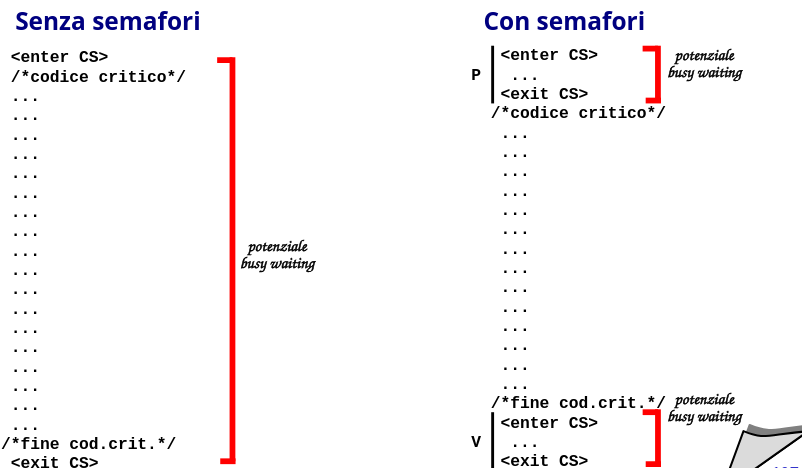
\includegraphics[width=0.7\textwidth]{img/semafori.png}
\end{figure} \\
\vspace{3em} \\
\textbf{Semafori binari\\}
Variante dei semafori in cui il valore può assumere solo i valori 0 e 1.
\begin{align*}
  0  \leq n_v + init - n_p \leq 1 \\
  0 \leq s.value \leq 1
\end{align*}
Servono a garantire mutua esclusione, semplificando il lavoro del programmatore. Analizziamo il codice:
\begin{lstlisting}[language=C]
class BinarySemaphore {
  private int value;
  Queue queue0 = new Queue();
  Queue queue1 = new Queue();
  BinarySemaphore() { value = 1;}
\end{lstlisting}
\begin{minipage}{0.48\textwidth}
\begin{lstlisting}[language=C]
void P() {
  [enter CS]
  int pid = <process id>;
  if (value == 0) {
    queue0.enqueue(pid);
    suspend(pid);
  } else if (queue1.size() > 0) {
    int pid = queue1.dequeue();
    wakeup(pid);
  } else
    value--;
  [exit CS]
}
\end{lstlisting}
\end{minipage} 
\begin{minipage}{0.70\textwidth}
\begin{lstlisting}[language=C]
void V() {
  [enter CS]
  int pid = <process id>;
  if (value == 1) {
    queue1.enqueue(pid);
    suspend(pid);
  } else if (queue0.size() > 0) {
    int pid = queue0.dequeue();
    wakeup(pid);
  } else
    value++;
  [exit CS]
}
\end{lstlisting}
\end{minipage} \\
\vspace{12em} \\
Possiamo definire i semafori generali attraverso semafori binari \\
\begin{minipage}{0.48\textwidth}
\begin{lstlisting}[language=C]
class Semaphore {
  private BinarySemaphore mutex(1);
  int value;
  QueueOfBinSem queue = new QueueOfBinSem();
  Semaphore(int v) { // +fail if v < 0
  value = v;}
\end{lstlisting}
\end{minipage}
\begin{itemize}
  \item un semaforo \texttt{mutex} per garantire mutua esclusione sulle variabili
  \item un semaforo privato creato in allocazione dinamica per ogni processo che partecipa
  \item una coda per garantire fairness
\end{itemize}
\begin{minipage}{0.48\textwidth}
\begin{lstlisting}[language=C]
void P() {
  mutex.P();
  if (value > 0) {
    value--;
    mutex.V();
  } else {
    S = new BinarySemaphore(0);
    queue.enqueue(S);
    mutex.V();
    S.P();
    free(S);
  }
}
\end{lstlisting}
\end{minipage}
\begin{minipage}{0.48\textwidth}
\begin{lstlisting}[language=C]
void V() {
  mutex.P();
  if (queue.empty())
    value++;
  else {
    BinarySemaphore s = queue.dequeue();
    s.V();
  }
  mutex.V();
}
\end{lstlisting}
\end{minipage}
\begin{lstlisting}[language=C]
class BinarySemaphore {
  private Semaphore s0, s1;
  int value;
  BinarySemaphore(int v) { // +fail if v not in {0,1}
  S0 = new semaphore(v)
  S1 = new semaphore(1-v)
}
  void P(void) {
    S0.P();
    S1.V();
  }
  void V(void) {
    S1.P();
    S0.V();
  }
}
\end{lstlisting}
\vspace{3em} 
\textbf{Produttore/Consumatore\\}
Esiste un processo "produttore" Producer che genera valori (record, caratteri, oggetti, etc.) e vuole trasferirli a un processo "consumatore" Consumer che prende i valori generati e li "consuma". La comunicazioni avviene attraverso una variabile condivisa.
\begin{lstlisting}[language=C]
shared Object buffer;
Semaphore empty =
  new Semaphore(1);
Semaphore full =
  new Semaphore(0);
\end{lstlisting}
\begin{minipage}{0.48\textwidth}
\begin{lstlisting}[language=C]
process Producer {
  while (true) {
    Object val = produce();
    empty.P();
    buffer = val;
    full.V();
  }
}
\end{lstlisting}
\end{minipage}
\begin{minipage}{0.48\textwidth}
\begin{lstlisting}[language=C]
process Consumer {
  while (true) {
    full.P();
    Object val = buffer;
    empty.V();
    consume(val);
  }
}
\end{lstlisting}
\end{minipage}\\
\vspace{3em} \\
\textbf{Buffer limitato\\}
In questo caso, però, lo scambio tra produttore e consumatore non avviene tramite un singolo elemento, ma tramite un buffer di dimensione limitata, i.e. un vettore di elementi.
\begin{lstlisting}[language=C]
Queue q(maxsize = SIZE);
Semaphore empty =
  new Semaphore(SIZE);
Semaphore full =
  new Semaphore(0);
Semaphore mutex =
  new Semaphore(1);
\end{lstlisting}
\begin{minipage}{0.48\textwidth}
\begin{lstlisting}[language=C]
process Producer {
  while (true) {
    Object val = produce();
    empty.P();
    mutex.P();
    q.enqueue(val);
    mutex.V();
    full.V();
  }
}
\end{lstlisting}
\end{minipage}
\begin{minipage}{0.48\textwidth}
\begin{lstlisting}[language=C]
process Consumer {
  while (true) {
    Object val;
    full.P();
    mutex.P();
    val = q.dequeue();
    mutex.V();
    empty.V();
    consume(val);
  }
}
\end{lstlisting}
\end{minipage}\\
\vspace{15em} \\
È possibile utlizzare il codice precedente con produttori e consumatori multipli? \\
Il \textbf{problema dei filosofi a cena} è un classico esempio di \textit{sincronizzazione concorrente}:
\begin{itemize}
    \item Ci sono 5 filosofi seduti attorno a un tavolo circolare.
    \item Tra ogni coppia di filosofi c’è una bacchetta.
    \item Ogni filosofo alterna due attività: \textbf{pensare} ed \textbf{mangiare}.
    \item Per mangiare, un filosofo ha bisogno \textbf{di entrambe le bacchette adiacenti}.
    \item Se tutti i filosofi prendono contemporaneamente la bacchetta alla loro destra (o sinistra), nessuno potrà mai prendere la seconda bacchetta, creando un \textbf{deadlock} (attesa circolare infinita).
\end{itemize}
\begin{lstlisting}[language=C]
Semaphore chopsticks = { new Semaphore(1), ..., new Semaphore(1) };
\end{lstlisting}
\begin{minipage}{0.58\textwidth}
\begin{lstlisting}[language=C]
process Philo[i] { /* i = 0...3 */
  while (true) {
    think
    chopstick[i].P();
    chopstick[i+1].P();
    eat
    chopstick[i].V();
    chopstick[i+1].V();
  }
}
\end{lstlisting}
\end{minipage}
\begin{minipage}{0.48\textwidth}
\begin{lstlisting}[language=C]
process Philo[4] {
  while (true) {
    think
    chopstick[0].P();
    chopstick[4].P();
    eat
    chopstick[0].V();
    chopstick[4].V();
  }
}
\end{lstlisting}
\end{minipage}\\
La soluzione si basa su due concetti chiave:

\begin{enumerate}
    \item \textbf{Eliminare l’attesa circolare:} rompere la simmetria nella sequenza di presa delle bacchette, evitando che tutti seguano lo stesso ordine.
    \item \textbf{Rompere la simmetria con un filosofo ``mancino'':} tutti i filosofi prendono prima la bacchetta alla loro destra e poi quella alla sinistra, \textbf{tranne uno} che fa il contrario. Questo garantisce che almeno un filosofo possa mangiare, liberando le bacchette per gli altri.
\end{enumerate}

\subsection*{Implementazione con semafori}
\begin{itemize}
    \item Ogni bacchetta è rappresentata da un \textbf{semaforo binario} inizializzato a 1.
    \item I filosofi ``destri'' prendono prima la bacchetta sinistra, poi quella destra.
    \item Il filosofo ``mancino'' prende prima la bacchetta destra, poi quella sinistra.
    \item Dopo aver mangiato, ciascun filosofo rilascia entrambe le bacchette.
\end{itemize}

\noindent
\textbf{Vantaggio:} questa semplice modifica evita il deadlock pur mantenendo il codice semplice. \\
\vspace{3em} \\
\textbf{Lettori e scrittori\\}
Un database è condiviso tra un certo numero di processi di due tipologie
\begin{itemize}
  \item lettori: accedono al database per leggerne il contenuto
  \item scrittori: accedono al database per aggiornarne il contenuto
\end{itemize}
Se uno scrittore sta scrivendo il database è in mutua eslusione, mentre per la lettura abbiamo più lettori contemporaneamente. \\
Questo avviene attraverso \textbf{classi di processi} cosi la mutua esclusione e la condivisione possono coesistere. \\
\begin{minipage}{0.48\textwidth}
\begin{lstlisting}[language=C]
process Reader {
  while (true) {
    startRead();
    read the database
    endRead();
  }
}
\end{lstlisting}
\end{minipage}
\hfill
\begin{minipage}{0.48\textwidth}
\begin{lstlisting}[language=C]
process Writer {
  while (true) {
  startWrite();
  write the database
  endWrite();
  }
}
\end{lstlisting}
\end{minipage} \\
Quindi un lettore potrà leggere in qualsiasi momento tranne che se uno scrittore stia scrivendo, mentre uno scrittore deve aspettare che i lettori finiscano di leggere (minima attesa possibile)
\begin{lstlisting}[language=C]
/* Variabili condivise */
int nr = 0;
Semaphore rw = new Semaphore(1);
Semaphore mutex = new Semaphore(1);

void startRead() {
  mutex.P();
  if (nr == 0)
    rw.P();
  nr++;
  mutex.V();
}

void startWrite() {
  rw.P();
}

void endRead() {
  mutex.P();
  nr--;
  if (nr == 0)
    rw.V();
  mutex.V();
}

void endWrite() {
  rw.V();
}
\end{lstlisting}
Questa soluzione però limita molto i lettori. Come possiamo risolverla? \\
Introduciamo una notazione prima di arrivare alla soluzione finale:
\begin{itemize}
  \item \textbf{B} condizione booleana
  \item \textbf{S} uno statement 
  \item $\langle S \rangle $: $\quad$ esegui lo statement $S$ in modo atomico
  \item $\langle \text{await}(B) \to S$ attendi (atomico) finchè $B$ non si vero e quindi esegui (amotico) $S$ \\
  Quindi quando $S$ è esegito $B$ è verificata
\end{itemize}
Quindi la logica sarebbe
\begin{lstlisting}[language=C]
< S >
  mutex.P();
  S;
  SIGNAL();

< await(Bi) -> Si>
  mutex.P();
  if (!Bi) {
    waiting[i]++;
    mutex.V();
    sem[i].P();
    waiting[i]--;
  }
  Si;
  SIGNAL();

void SIGNAL() //non deterministica
{
  if (B0 && waiting[0]>0)
    sem[0].V();
  if (B1 && waiting[1]>0)
    sem[1].V();
   ...
   if (Bn-1 && waiting[n-1]>0)
    sem[n-1].V();
  if (!(B0 && waiting[0]>0) && !(B1 && waiting[1]>0) && ... 
   !(Bn-1 && waiting[n-1]>0) )
      mutex.V();
}
\end{lstlisting}
Questa trasformazione si chiama passaggio del testimone (“\textit{passing the baton}”). Ovvero SIGNAL verifica se esiste un processo, fra quelli in attesa, che possono proseguire se esiste, "gli passa il testimone" (la mutua esclusione) altrimenti la rilascia. Si definisce come un semaforo binario suddiviso tra i vari semafori (split binary semaphore).
\begin{lstlisting}[language=C]
/* Introduced by transformation */
Semaphore mutex = new Semaphore(1); /* Mutual exclusion */
Semaphore semr = new Semaphore(0); /* Reader semaphore */
Semaphore semw = new Semaphore(0); /* Writer semaphore */
int waitingr = 0; /* Number of waiting reader */
int waitingw = 0; /* Number of waiting writer */
/* Problem variables */
int nr = 0; /* Number of current readers */
int nw = 0; /* Number of current writers */
\end{lstlisting}
\begin{minipage}{0.48\textwidth}
\begin{lstlisting}[language=C]
process Reader {
  while (true) {
    mutex.P();
    if (nw > 0) {
      waitingr++;
      mutex.V();
      semr.P();
      waitingr--;
  }
  nr++;
  SIGNAL();
  read the database
  mutex.P();
  nr--;
  SIGNAL();
}
\end{lstlisting}
\end{minipage}
\begin{minipage}{0.48\textwidth}
\begin{lstlisting}[language=C]
process Writer {
  while (true) {
    mutex.P();
    if (nr >0 || nw > 0) {
      waitingw++;
      mutex.V();
      semw.P();
      waitingw--;
    }
  nw++;
  SIGNAL();
  write the database
  mutex.P();
  nw--;
  SIGNAL();
}
\end{lstlisting}
\end{minipage} \\
\begin{lstlisting}[language=C]
void SIGNAL() {
  if ( (nw == 0) && waitingr > 0)
    semr.V();
  if ( (nw == 0 && nr == 0) && waitingw > 0)
    semw.V();
  if ( !( (nw == 0) && waitingr > 0 ) &&
  !( (nw == 0 && nr == 0) && waitingw > 0 ) ){ 
    mutex.V() 
  }
}
\end{lstlisting} 
Vediamo ora: R/W trasformato (SIGNAL ridotto, non-determinismo eliminato) \\
\begin{minipage}{0.48\textwidth}
\begin{lstlisting}[language=C]
process Reader {
  while (true) {
    mutex.P();
    if (nw > 0) {
      waitingr++;
      mutex.V();
      semr.P();
      Waitingr--;
  }
  nr++;
  if (waitingr > 0)
    semr.V();
  else
    mutex.V();
  read the database
  mutex.P();
  nr--;
  if (nr == 0 && waitingw > 0)
    semw.V();
  else
    mutex.V();
}
\end{lstlisting}
\end{minipage}
\begin{minipage}{0.48\textwidth}
\begin{lstlisting}[language=C]
process Writer {
  while (true) {
    mutex.P();
    if (nr > 0 || nw > 0) {
      waitingw++;
      mutex.V();
      semw.P();
      Waitingw--;
    }
    Nw++;
    mutex.V();
    write the database
    mutex.P();
    nw--;
    if (waitingr > 0)
      semr.V();
    else if (waitingw > 0)
      semw.V();
    else
      mutex.V();
  }
}
\end{lstlisting}
\end{minipage} \\
Queste versioni danno priorità ai lettori e quindi abbiamo starvation per gli scrittori. Vediamo ora la versione senza la starvation \\
\begin{minipage}{0.48\textwidth}
\begin{lstlisting}[language=C]
process Reader {
  while (true) {
    mutex.P();
    if (nw > 0 || waitingw > 0){ 
      waitingr++; mutex.V();
      semr.P(); waitingr--;
    }
    nr++;
    if (waitingr > 0)
      semr.V();
    else
      mutex.V();
    read the database
    mutex.P();
    nr--;
    if (nr == 0 && waitingw > 0)
      semw.V();
    else
      mutex.V();
}
\end{lstlisting}
\end{minipage} 
\begin{minipage}{0.48\textwidth}
\begin{lstlisting}[language=C]
process Writer {
  while (true) {
    mutex.P();
    if (nr > 0 || nw > 0) {
      waitingw++; mutex.V();
      semw.P(); waitingw--;
    }
    nw++;
    mutex.V();
    write the database
    mutex.P();
    nw--;
    if (waitingr > 0)
      semr.V();
    else if (waitingw>0)
      semw.V();
    else
      mutex.V();
  }
}
\end{lstlisting}
\end{minipage} \\
\vspace{2em} \\
\textbf{Il barbiere addormentato} \\
Un negozio di barbiere ha un barbiere, una poltrona da barbiere e n sedie per i clienti in attesa. Quando non ci sono clienti il barbiere si mette sulla sedia da barbiere e si addormenta. Quando arriva un cliente, sveglia il barbiere addormentato e si fa tagliare i capelli sulla sedia da barbiere. Se arriva un cliente mentre il barbiere sta tagliando i capelli a un altro cliente, il cliente si mette in attesa su una delle sedie. Se tutte le sedie sono occupate, il cliente se ne va scocciato! \\
\vspace{2em} \\
Da come abbiamo visto i semafori hanno diverse falle, a partire dagli errori "banali" del programmatore alla leggibilità scarsa del codice. Che alternative abbiamo?
\subsection{Monitor}
Un monitor è un modulo software che consiste di:
\begin{itemize}
  \item dati locali
  \item sequenza di inizializzazione
\end{itemize}
Le caratteristiche sono
\begin{itemize}
  \item i dati locali sono accessibili solo alle procedure del modulo stesso
  \item un processo entra in un monitor invocando una delle sue procedure
  \item solo un processo alla volta può essere all'interno del monitor, gli altri processi che invocano il monitor sono sospesi
\end{itemize}
Vediamo una "pseudo-sintassi" della struttura
\begin{lstlisting}[language=C]
monitor name {
  variable declarations...
  procedure entry type procedurename1(args...) {
    ...
  }
  type procedurename2(args...) {
    ...
  }
  name(args...) {
    ...
  }
}
\end{lstlisting}
A livello tecnico la programmazione ad oggetti ci semplifica la vita 
infatti la inizializzazione coincide con il costruttore
\begin{itemize}
  \item \texttt{Inizializzaione} = Costruttore
  \item \texttt{Procedure entry} = metodi pubblici dell'oggetto
  \item \texttt{Procedure normali} = metodi privati
  \item \texttt{Variabili locali} = variabili private 
\end{itemize}
Da come abbiamo detto solo un processo alla volta può essere all'interno del monitor, quindi questo ci fornisce un semplice strumento di mutua esclusione. \\
\vspace{5px} \\
Come logica definiamo
\begin{itemize}
  \item condition c;
  \item c.wait() \\
  attende il verificarsi della condizione, viene sospeso in una coda di attesa della condizione c
  \item c.signal() \\
  segnala che la condizione è vera, causa la riattivazione immediata di un processo
\end{itemize}
\begin{figure}[h] 
    \centering
    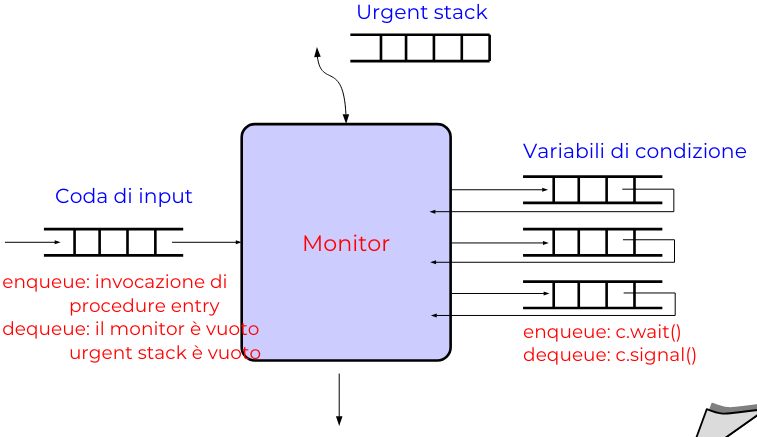
\includegraphics[width=0.7\textwidth]{img/monitor.png}
\end{figure} 
\textbf{Signal urgent} (SU) è la politica "classica" di signaling. \\
Possiamo anche implementare i \textbf{semafori} con questa logica.
\begin{lstlisting}[language=C]
monitor Semaphore {
  int value;
  condition c; /* value > 0 */
  procedure entry void P() {
    if (value == 0)
    c.wait();
    value--;
  }
  procedure entry void V() {
    value++;
    c.signal();
  }
  Semaphore(int init) {
    value = init;
  }
}
\end{lstlisting}
E per il \textbf{R/W}? Vediamo la versione senza la starvation
\begin{lstlisting}[language=C]
monitor RWController
  int nr; /* number of readers */
  int nw; /* number of writers */
  condition okToRead; /* nw == 0 */
  condition okToWrite; /* nr == 0 && nw == 0 */

procedure entry void startRead() {
  if (nw > 0 || ww > 0) okToRead.wait();
  nr = nr + 1;
  okToRead.signal();
}
procedure entry void endRead() {
  nr = nr - 1;
  if (nr == 0) okToWrite.signal();
}
procedure entry void startWrite() {
  if (nr > 0 || nw > 0) { ww++; okToWrite.wait(); ww--; }
  nw = nw + 1;
}
procedure entry void endWrite() {
  nw = nw - 1;
  okToRead.signal();
  if (nr == 0) okToWrite.signal();
}
\end{lstlisting}
\vspace{2em}
Invece per \textbf{Produttore / Consumatore}? Abbiamo anche quella
\begin{lstlisting}[language=C]
monitor PCController {
  Object buffer;
  condition empty;
  condition full;
  boolean isFull;
  PCController() {
    isFull=false;
  }
  
  procedure entry Object read() {
  if (!isFull)
    full.wait();
  int retvalue = buffer;
  isFull = false;
  empty.signal();
  return retvalue;
  }
  
  procedure entry void write(int val){
  if (isFull)
    empty.wait();
  buffer = val;
  isFull = true;
  full.signal();
  }
}
\end{lstlisting}
\begin{minipage}{0.48\textwidth}
\begin{lstlisting}[language=C]
process Producer {
  Object x;
  while (true) {
    x = produce();
    pcController.write(x);
  }
}
\end{lstlisting}
\end{minipage}
\begin{minipage}{0.48\textwidth}
\begin{lstlisting}[language=C]
process Consumer {
  Object x;
  while (true) {
    x = pcController.read();
    consume(x);
  }
}
\end{lstlisting}
\end{minipage} \\
\vspace{2em} \\
\textbf{Buffer limitato tramite Monitor}
\begin{lstlisting}[language=C]
monitor PCController {
  QueueOfObj q;
  int maxsz
  condition okRead; //q.size > 0.
  condition okWrite;//q.size < maxsz
  PCController(int size) {
    maxsz = size;
  }
\end{lstlisting}
\begin{minipage}{0.58\textwidth}
\begin{lstlisting}[language=C]
procedure entry void write(Obj val)
{
  if (q.size() >= maxsz)
    okWrite.wait();
  q.enqueue(val);
  okRead.signal();
}
\end{lstlisting}
\end{minipage}
\hfill
\begin{minipage}{0.48\textwidth}
\begin{lstlisting}[language=C]
procedure entry Object read() {
  if (q.size() == 0)
    okRead.wait();
  Obj retval = q.dequeue();
  okWrite.signal();
  return retval;
}
\end{lstlisting}
\end{minipage} \\
\vspace{2em} \\
\textbf{Filosofi a cena}
\begin{lstlisting}[language=C]
monitor DPController {
  condition unusedchopstick[5];
  boolean chopstick[5];
  procedure entry void startEating(int i) {
    if (chopstick[i])
      unusedchopstick[i].wait();
    chopstick[i] = true;
    if (chopstick[(i+1)%5])
      unusedchopstick[(i+1)%5].wait();
    chopstick[(i+1)%5] = true;
  }
  procedure entry void finishEating(int i) {
    chopstick[i] = false;
    chopstick[(i+1)%5] = false;
    unusedchopstick[i].signal();
    unusedchopstick[(i+1)%5].signal();
  }
}

monitor chopstick[i] {
  boolean inuse = false;
  condition free;
  procedure entry void pickup() {
    if (inuse)
    free.wait();
    inuse = true;
  }
  procedure entry void putdown() {
    inuse = false;
    free.signal();
  }
}

process Philo[i] {
  while (true) {
    think
    chopstick[MIN(i,(i+1)%5)].pickup();
    chopstick[MAX(i,(i+1)%5)].pickup();
    eat
    chopstick[MIN(i,(i+1)%5)].putdown();
    chopstick[MAX(i,(i+1)%5)].putdown();
  }
}
\end{lstlisting} 
\vspace{2em} 
Ma come li implementiamo i monitor? \\
\begin{itemize}
  \item Uno stack (per urgent)
  \item Una queue (per waiting queue)
  \item Un semaforo 
\end{itemize}
E poi il codice della struttura e relative funzioni.
\vspace{2em} 
\subsection{Message passing}
Fino ad ora abbiamo visto metodi per sincronizzare i processi basati sulla memoria, ora ragioniamo con lo scambio di messaggi, e non più semplici segnali.
\begin{figure}[h] 
    \centering
    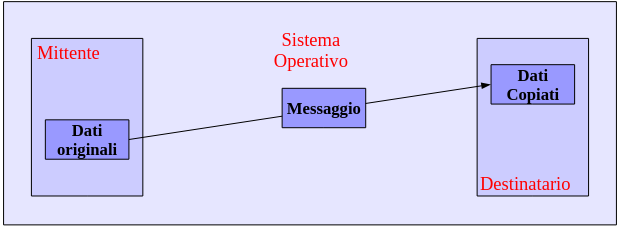
\includegraphics[width=0.7\textwidth]{img/message.png}
\end{figure} 
\begin{itemize}
  \item send: "spedire" un messaggio ad un processo destinatario
  \item receive: "ricevere" un messaggio da un processo mittente
\end{itemize}
Abbiamo 3 tipologie di message passing
\begin{itemize}
  \item MP sincrono
    \begin{itemize}
      \item send sincrona: il mittente spedisce il messaggio al processo, restando bloccato fino a quando il destinatario non riceve il messaggio
      \item receive bloccante: il destinatario riceve un messaggio dal processo send. Se il bmittente non ha ancora spedito alcun messaggio, il destinatario si blocca in attesa di ricevere un messaggio
    \end{itemize}
  \item MP asincrono
    \begin{itemize}
      \item send asincrono: il mittente spedisce il messaggio al processo destinatario, senza bloccarsi in attesa che il destinatario riceva il messaggio
      \item receive bloccante: il destinatario riceve un messaggio dal processo send. Se il mittente non ha ancora spedito alcun messaggio, il destinatario si blocca in attesa di ricevere un messaggio
    \end{itemize}
  \item MP completamente asincrono
    \begin{itemize}
      \item send asincrona: il mittente spedisce il messaggio al processo destinatario, senza bloccarsi in attesa che il destinatario riceva il messaggio
      \item receive non bloccante: il destinatario riceve un messaggio dal processo send. Se il mittente non ha ancora spedito alcun messaggio, la nb-receive (la sua funzione) termina ritornando un messaggio "nullo"
    \end{itemize}
\end{itemize}
\begin{figure}[h] 
    \centering
    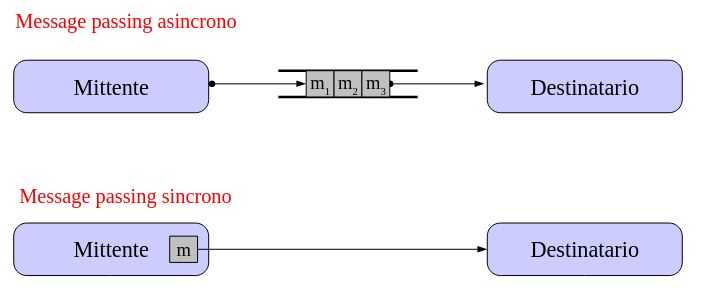
\includegraphics[width=0.7\textwidth]{img/asincrono.png}
\end{figure} 
Noi utilizzeremo un message passing \textbf{asincrono} con \texttt{send}, \texttt{receive}, \texttt{reply}. \\
Vediamo quindi un MP asincrono dato quello sincrono (senza gestione ANY)
\begin{lstlisting}[language=C]
/* p is the calling process */
void asend(msg_t m, pid_t dst) {
  ssend("SND(m,getpid(),dst)", server);
}
msg_t areceive(pid_t snd) {
  ssend("RCV(getpid(),snd)", server);
  msg_t m = sreceive(server);
  return m;
}
process server {
  /* One element x process pair */
  int[][] waiting;
  Queue[][] queue;
  while (true) {
    handleMessage();
  }
}
void handleMessage() {
  msg = sreceive(0);
  if (msg == <SND(m,p,q)>) {
    if (waiting[p,q]>0) {
      ssend(m, q);
      waiting[p,q]--;
    } else {
      queue[p,q].add(m);
    }
  } else if (msg == <RCV(q,p)>) {
    if (queue[p,q].isEmpty()) {
      waiting[p,q]++;
    } else {
      m = queue[p,q].remove();
      ssend(m, q);
    }
  }
}
\end{lstlisting}
\vspace{2em}
\textbf{Message Passing - Filosofi a cena}
\begin{lstlisting}[language=C]
process Philo[i] {
  while (true) {
    think
    asend(<PICKUP,i>, chopstick[MIN(i, (i+1)%5)]);
    msg = areceive(chopstick[MIN(i, (i+1)%5)]);
    asend(<PICKUP,i>, chopstick[MAX(i, (i+1)%5)]);
    msg = areceive(chopstick[MAX(i, (i+1)%5)]);
    eat
    asend(<PUTDOWN,i>, chopstick[MIN(i, (i+1)%5)]);
    asend(<PUTDOWN,i>, chopstick[MAX(i, (i+1)%5)]);
  }
}
process chopstick[i] {
  boolean free = true;
  Queue queue = new Queue();
  while (true) {
    handleRequests();
  }
}
void handleRequests() {
  msg = areceive(0);
  if (msg == <PICKUP,j>) {
    if (free) {
      free = false;
      asend(ACK, philo[j]);
    } else {
    queue.add(j);
    }
  } 
  else if (msg == <PUTDOWN, j>) {
      if (queue.isEmpty()) {
      free = true;
    } else {
    k = queue.remove();
    asend(ACK, philo[k]);
    }
  }
}
\end{lstlisting}
\vspace{2em} 
\textbf{Message Passing - Produttori e consumatori}
\begin{lstlisting}[language=C]
process PCmanager {
  Object x;
  while (true) {
    x = sreceive(Producer);
    ssend(x, Consumer);
  }
}
\end{lstlisting}
\begin{minipage}{0.48\textwidth}
\begin{lstlisting}[language=C]
process Consumer{
  Object x;
  while (true) {
    x = sreceive(PCmanager);
    consume(x);
  }
}
\end{lstlisting}
\end{minipage}
\hfill
\begin{minipage}{0.48\textwidth}
\begin{lstlisting}[language=C]
process PCmanager {
  Object x;
  while (true) {
    x = sreceive(Producer);
    ssend(x, Consumer);
  }
}
\end{lstlisting}
\end{minipage}
\vspace{2em} \\
\subsection{Conclusioni}
\begin{itemize}
  \item Sezioni critiche: realizzare mutua esclusione in sistemi mono e multiprocessore all'interno del sistema operativo stesso. (troppo basso livello)
  \item Semafori: primitiva di sincronizzazione, effettivamente offerta dai S.O. (troppo basso)
  \item Monitor: meccanismi integrati nei linguaggi di programmazione
  \item Message passing: meccanismo più diffuso, può essere poco efficiente
\end{itemize}
Si possono tracciare le seguenti classi di paradigmi:
\begin{itemize}
  \item Metodi a memoria condivisa: 
  \begin{itemize}
    \item semafori, semafori binari, monitor (stesso potere espressivo)
    \item dekker e peterson, Test\&Set necessitano di busy waiting
  \end{itemize}
    \item Metodi a memoria privata: 
  \begin{itemize}
    \item message passing asincrono ha maggiore potere espressivo
    \item message passing sincrono
  \end{itemize}
\end{itemize}
\textit{Ricorda}: si dice che il paradigma di programmazione $A$ è espressivo almeno quanto il paradigma di programmazione $B$ (e si scrive $A \geq B$) quando è possibile esprimere ogni programma scritto con $B$ mediante $A$. Ovvero, quando è possibile scrivere una libreria che consenta di implementare le chiamate di un paradigma $B$ esprimendole in termini di $A$ si avrà $A \geq B$.
\pagebreak
\section{Generale}
\subsection{Architettura di un calcolatore}
Ripassiamo la architettura di Von Neumann
\begin{figure}[h] % [h] = qui (here)
    \centering
    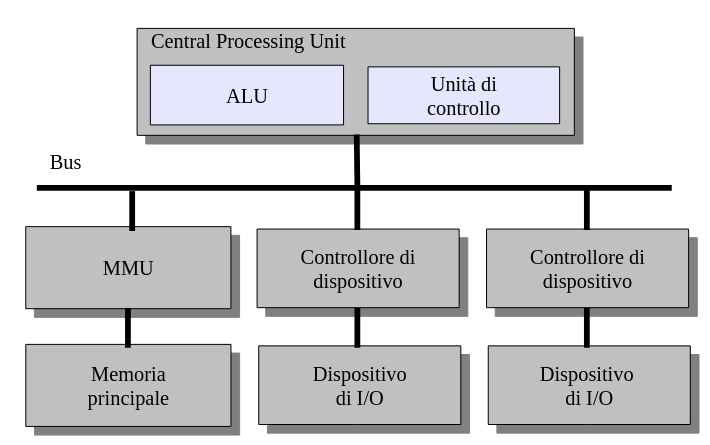
\includegraphics[width=0.7\textwidth]{img/von.png}
\end{figure} \\
Definiamo
\begin{itemize}
  \item Device: hardware
  \item Device controller: scheda elettronica che controlla il dispositivo (hardware)
  \item Device driver: software
  \item Memory management unit: unita controllo memoria (hardware)
  \item Memory manager: parte del S.O. che gestisce la MMU (software)
\end{itemize}
\paragraph{Interrupt} Meccanismo che interrompe il ciclo della CPU. Permettono al S.O.di intervenire durante l'esecuzione di un programma.
\begin{itemize}
  \item Interrupt hardware: eventi asincroni, non causati dal processo in esecuzione. (I/O, interval time)
  \item Interrupt software (trap): causato del programma. (divisione per 0, chiamate di system call) 
\end{itemize}
Gli interrupt sono inviati al/ai processori, o alle schede controller del dispositivo. \\
Cosa succedere dopo aver chiamato un interrupt?
\begin{itemize}
  \item 1) Invio di \textit{interrupt request} al processore
  \item 2) Il processore sospende le operazioni, salta ad un indirizzo specifico (interrupt handler)
  \item 3) Qua nel interrupt handler gestiamo correttamente l'interrupt, ritorniamo il controllo al processo interrotto (o ad un altro processo)
  \item 4) Il processore riprende l'esecuzione, come se non fosse successo niente
\end{itemize}
\begin{figure}[H]
    \centering
    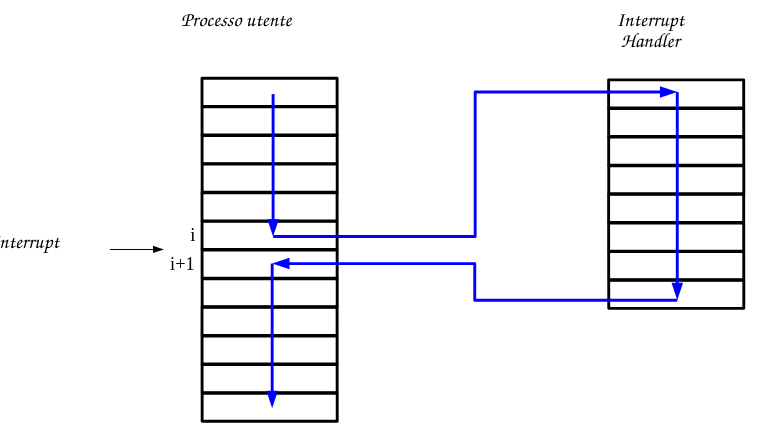
\includegraphics[width=0.7\textwidth]{img/interrupt.png}
\end{figure} 
E nel caso se avessimo più interrupt? 
\begin{itemize}
  \item Disabilitazione degli interrupt: se durante l'esecuzione di un interrupt handler riceviamo un altro interrupt lo ignoriamo fino ad avere finito il nostro interrupt handler per poi eseguirlo dopo.
  \begin{figure}[H]
    \centering
    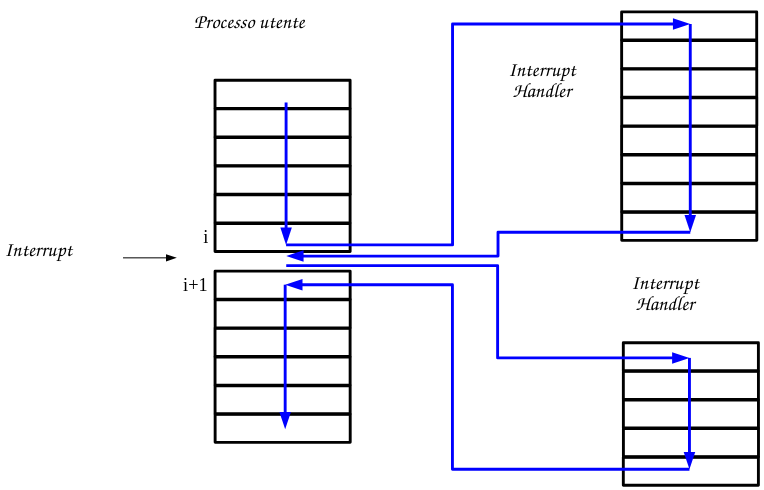
\includegraphics[width=0.6\textwidth]{img/dis.png}
\end{figure} 
  \item Interrupt annidati: Abbiamo delle priorità, e uno inferiore può essere interrotto da uno di priorità maggiore. 
    \begin{figure}[H]
    \centering
    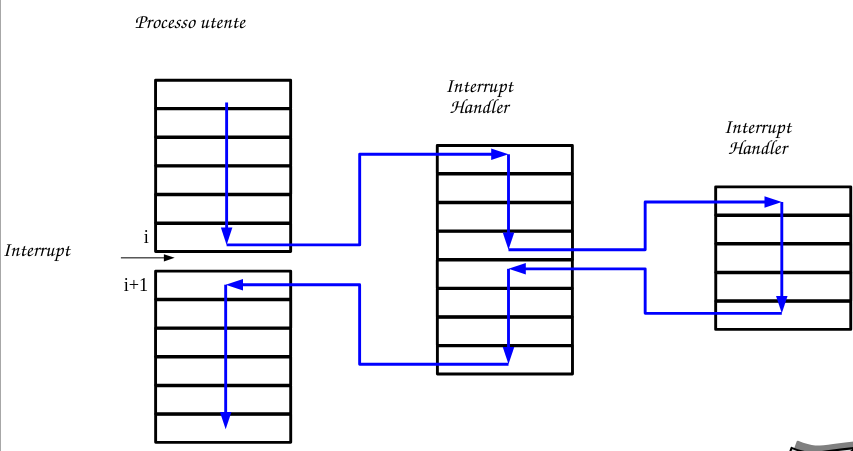
\includegraphics[width=0.6\textwidth]{img/annidati.png}
\end{figure} 
\end{itemize}
\paragraph{Comunicazione fra processore e dispositivi di I/O} Il controller fa da tramite tra il dispotivo I/O e il processore. Come lo implementiamo?
\begin{itemize}
  \item Programmed I/O (obsoleto): La CPU carica nel controller la richiesta, il controller esegue e si copia in un suo buffer il risultato. Nel frattempo il SO controlla quando l'operazione è stata completata. Si segna in appositi suoi registri del controller che l'operazione è stata completata. La CPU copia i dati nella memoria.
  \item Interrupt-Driven I/O: La CPU carica nel controller la richiesta, il SO sospende il processo e nel frattempo ne esegue un altro. Il controller nel frattempo esegue, copia nel suo buffer e segnala alla CPU via un interrupt il completamento. La CPU copia i dati dal buffer alla memoria. 
\end{itemize}
\vspace{1px}
\textbf{Direct Memory Access (DMA)} Il controller del dispositivo legge/scrive i dati direttamente dalla memoria centrale, senza passare dalla CPU. Il SO specifica l'indirizzo di memoria. \\
\vspace{1px}\\
\textbf{Memoria} Insieme ai registri è l'unico spazio di memoria che il processore può accedervi direttamente, nei sistemi moderni abbiamo anche la MMU che permette l'accesso modificando gli indirizzi logici in indirizzi fisici. \\
\vspace{1px}\\
\textbf{Memory Mapped I/O} Tramite il bus di sistema mappiamo i dati del dispositivo tramite indirizzi direttamente accesibili. La lettura/scrittura sul bus comporta il trasferimento di dati da o verso il dispositivo. Tutto questo necessita tecniche di sincronizzazione di accesso. \\
\vspace{1px}\\
\textbf{Dischi} Consentono la memorizzazione non volatile dei dati. Accesso random diretto. \\
Attraverso il controller possiamo:
\begin{itemize}
  \item READ(head, sector)
  \item WRITE(head, sector)
  \item SEEK(cylinder): spostamento fisico della testina da un cilindro all'altro.
\end{itemize}
\vspace{1px}
    \begin{figure}[H]
    \centering
    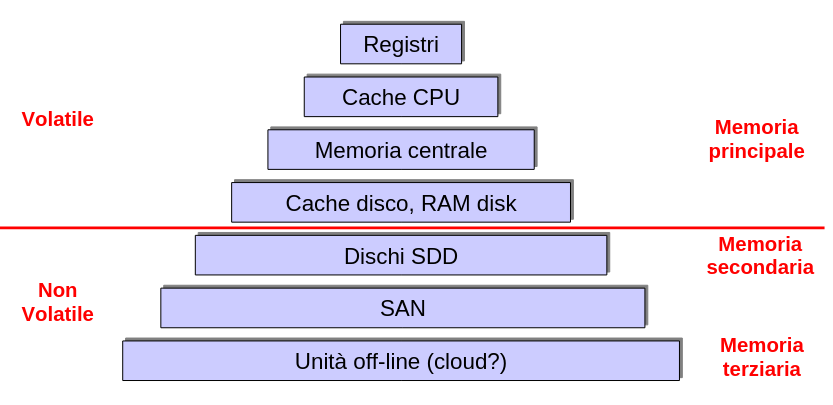
\includegraphics[width=0.7\textwidth]{img/memorie.png}
\end{figure} 
\textbf{Cache} Memorizzare parzialmente i dati di una memoria in una seconda più costosa ma più efficiente. Il caching lo troviamo nella DRAM attraverso la memoria bipolare (L1, L2), cache su disco fisso (cache HW), cache di file system remoti tramite file sistem locali (cache SW). Bisogna però avere il giusto algoritmo di caching che permetta di garantire il maggior numero possibile di accessi. \\
\vspace{2em} \\
Nei sistemi multiprogramma e multiutente dobbiamo avere meccanismi di protezione per evitare che i processi concorrenti creino conflitto. Li creiamo via HW o SW?
\begin{itemize}
  \item Hardware:
  \begin{itemize}
      \item Kernel: i processi qua hanno tutte le istruzioni, incluse istruzioni privilegiate, per gestire il sistema
      \item Utente: i processi in modalità utente non hanno accesso alle istruzioni privilegiate
  \end{itemize}
\end{itemize}
Come funziona?
\begin{itemize}
  \item CPU modalità Kernel
  \item Caricamento del SO (bootstrap), ed sua esecuzione
  \item Quando abbiamo un processo utente cambiamo il valore del \textit{mode bit} (nel registro) e mettiamo la CPU modalità utente
  \item Quando riceviamo un interrupt passiamo a modalità kernel
\end{itemize}  
Per garantire anche la protezione della memoria utilizziamo il MMU, nel quale l'indirizzo logico viene tradotto in indirizzo fisico e nel caso di traduzione impossibile l'indirizzo viene protetto.
\subsection{Architettura dei sistemi operativi}
\subsubsection*{Gestione dei processi}
Un processo utilizza le risorse fornite dal computer per svolgere i propri compiti. Il SO si deve occupare di creazione/terminazione dei processi, sospensione/riattivazione, gestione deadlock, comunicazione fra i processi, sincronizzazione dei processi.
\subsubsection*{Gestione della memoria principale}
La RAM è un array di dati accessibile dalla CPU e controller I/O se DMA. Il SO deve tenere traccia della memoria utilizzata e da chi, allocare/deallocare, decidere i processi da caricare, usare memoria secondaria per amplicare la memoria primaria.
\subsubsection*{Gestione della memoria secondaria}
Il SO gestisce il partizionamento, RAID, ordinamento efficiente delle richieste (disk scheduling).
\subsubsection*{Gestione file system}
Un file system è composto da un insieme di file. Il SO si occupa della creazione/cancellazione dei file e directory, manipolazione file/directory, codifica del file system su una sequenza di blocchi.
\subsubsection*{Gestione dei dispositivi di I/O}
Driver per hw specifico, gestione del buffer delle informazioni e una interfaccia comune per gestione dei driver.
\subsubsection*{Supporto multiuser}
Abbiamo bisogno di un meccanismo di protezione per controllare gli accessi dei processi alle risorse del sistema e degli utenti. Il SO deve garantire la protezione come: garantire identità de proprietario del processo, gestire chi può fare cosa.
\subsubsection*{Networking}
Consente di far comunicare processi in esecuzione su più elaboratori, e condividere risorse. Questo attraverso a protocolli a basso livello (TCP/UDP, IP) o alto livello (NFS, SMB). \\
\vspace{2em}\\
\subsubsection{Struttura del SO}
Un SO deve tener conto di efficienza, manuntenibilità, espansibilità e modularità.
\begin{itemize}
  \item Struttura semplice (o senza struttura)\\
  Sono SO semplice che pian piano sono stati fatti update oltre lo scopo originale. Più o come una collezione di procedure che si chiamano a vicenda.
  \begin{figure}[H]
    \centering
    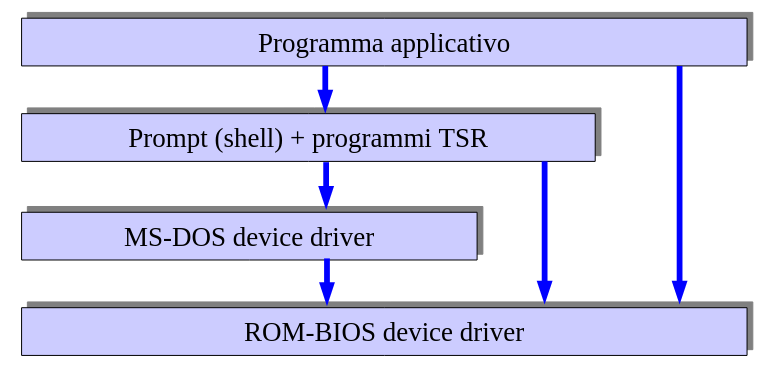
\includegraphics[width=0.7\textwidth]{img/dos.png}
\end{figure} 
MS-DOS: fortemente legato al hw, le interfaccie e i livelli di funzionalità non sono separati, quindi qualsiasi programma poteva fare I/O. Un crash del programma porta il crash del SO. \\
UNIX: poco più strutturato del precendete ma sempre legato al hw, suddiviso in kernel e programmi di sistema.
    \begin{figure}[H]
    \centering
    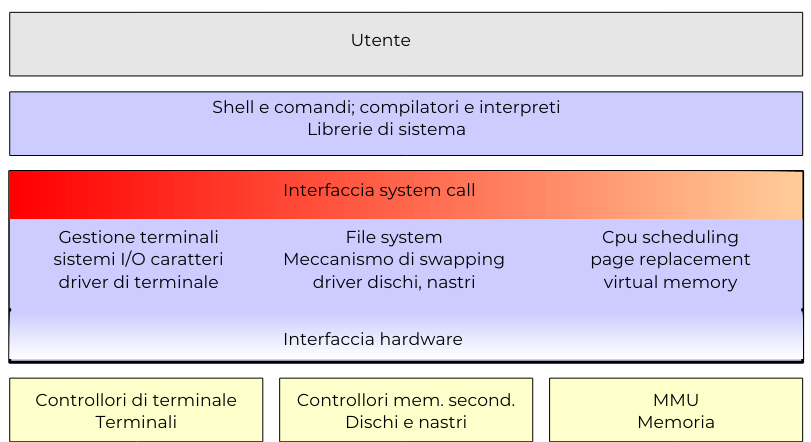
\includegraphics[width=0.7\textwidth]{img/unix.png}
\end{figure} 
  \item Struttura a strati\\
  Possiamo teorizzare un SO come un insieme di strati, questo ci da ampia modularità. Avere troppi strati però aggiunge molto overhead. Nella realtà si cerca di avere un numero limitato di strati.
\end{itemize}
\subsubsection{Software engineering del SO}
Filosofia che aiuta a progettare sistemi flessibili e manutenibili.
\begin{itemize}
  \item Politica: parte del sistema che prende le decisioni
  \item Meccanismo: parte che realizza materialmente le azioni decise dalla politica
\end{itemize}
Separandoli possiamo modificare una senza toccare l'altra e viceversa.\\
\paragraph{Microkernel} Si implementano nel kernel i soli meccanismi, delegando la gestione della politica a processi fuori dal kernel. \\
Cosa succede se li si unisce? Un semplice bug grafico può portare il crash di tutto il sistema.\\
\vspace{5px}\\
Come definiamo un kernel?
\begin{itemize}
  \item Kernel monolitici: unico insieme di procedure di gestione mutuamente coordinate e astrazioni dell’HW\\
  Attraverso le System calls implementiamo i servizi forniti dal kernel, che verranno poi eseguito in kernel mode in moduli. (Linux, FreeBSD UNIX)
  \item Micro kernel: semplici astrazioni dell’HW gestite e coordinate da un kernel minimale (tipo client/server, message passing)\\
  Rimuovendo dal kernel tutte le parti non essenziali e implementarle come processi a livello utente (per accedere ad un file, un processo interagisce con il processo gestore del file system). Alla base ci serve un meccanismo di comunizione \textit{message passing} che gestirà il microkernel. Tramite questo possiamo creare la maggior parte delle API dei SO moderni:
  \begin{lstlisting}
int open(char* file, ...)
{
msg = < OPEN, file, ... >;
send(msg, file-server);
fd = receive(file-server);
return fd;
}
  \end{lstlisting}
  \item Kernel ibridi: simili ai precedenti ma con più componenti eseguite in kernel space per efficienza.\\
  Sono microkernel che eseguono parte in kernel space, e message passing tra i moduli in user space (famiglia Windows NT)
\end{itemize}
\vspace{2em}
\subsubsection{Macchine virtuali}
Emuliamo il funzionamento del hw, possiamo eseguire qualsiasi SO.
\begin{figure}[h] % [h] = qui (here)
    \centering
    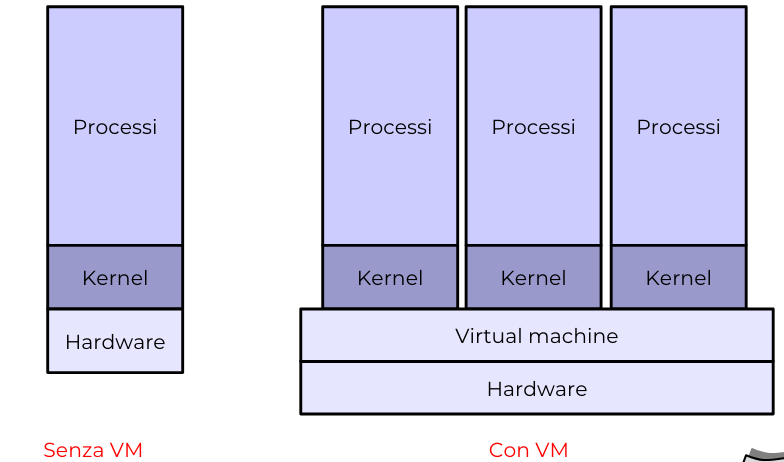
\includegraphics[width=0.7\textwidth]{img/vm.png}
\end{figure} \\
I vantaggi sono molteplici (emulazione archietture hw diverse, coesistenza di SO, sistemi monotask in multitask, ecc) ma a costo di una grande inefficienza e con alta difficoltà di condivisione delle risorse.\\
\vspace{2em}\\
\subsubsection{Namespace}
I namespace isolano le risorse in modo che i processi posano vedere solo quelle collegate a essi. (PID, NET, USER, ecc) Li troviamo in Linux, questi sono la base per i container ovvero un gruppo di processi che ha: immagine di file system privata, propria configurazione di rete, limiti di accesso alle risorse; tutto questo gestito da meccanismi di amministrazione a run-time (docker, containerd, ecc).
\subsection{Scheduling}
Un sistema operativo ha bisogno di strutture dati per mantenere informazioni sulle risorse gestite (processo, mem, principale/secondaria, dispositivi).\\
Queste strutture dati comprendono:
\begin{itemize}
  \item tabelle di memoria: allocazione memoria per il SO, sia principale che secondaria
  \item tabelle di I/O
  \item tabelle di filesystem: elenco dei dispositivi utilizzati per mantenere il file system, file aperti, ecc
  \item \textbf{tabelle dei processi}
\end{itemize}
\begin{figure}[h] % [h] = qui (here)
    \centering
    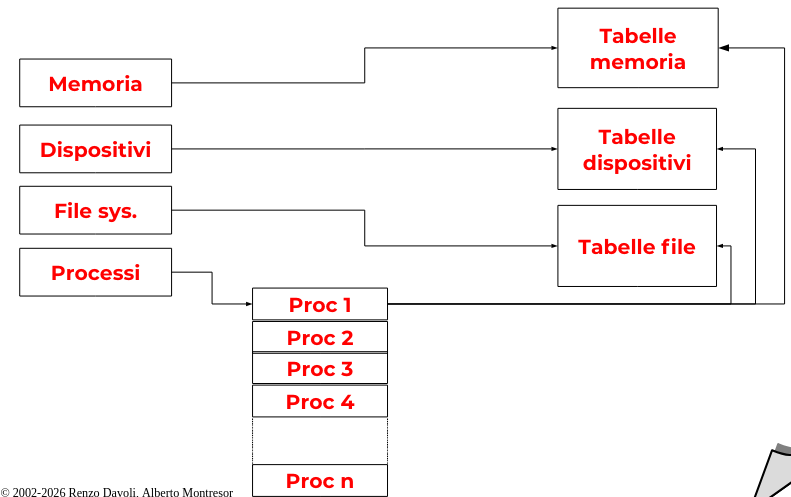
\includegraphics[width=0.7\textwidth]{img/sch.png}
\end{figure} 
Come è composto un processo per il SO?
\begin{itemize}
  \item il codice da eseguire
  \item i dati su cui operare
  \item uno stack di lavoro per la gestione di chiamate di funzione, passaggio di parametri e variabili locali
  \item un insieme di attributi contenenti tutte le informazioni necessarie per la gestione del processo stesso
\end{itemize}
Tutto questo si chiama \textbf{process control block} (PCB). Per gestire tutti i processi abbiamo una tabella di PCB (ogni processo ha 1 PCB). \\
Ogni PCB può essere suddiviso in
\begin{itemize}
  \item informazioni di identificazione di processo (pid, id utente, altri identificatori)
  \item informazioni di stato del processo (registri generali e speciali)
  \item informazioni di controllo del processo 
  \begin{itemize}
    \item informazioni di scheduling come esecuzione, attesa, ecc
    \item informazioni per algoritmo di scheduling utilizzato (es. priorità)
    \item informazioni gestione memoria
    \item informazioni relative alle risorse (file aperti, device, ecc)
    \item informazioni per interprocess communication (IPC) come semafori, stato segnali, ecc
  \end{itemize}
\end{itemize}
\subsubsection{Scheduler, processi e thread}
Lo \textbf{scheduler} è la componente più importante del SO, decide quale processo deve essere in esecuzione, interviene per richieste di I/O. Per questi ultimo come abiamo visto ogni volta che abbiamo un interrupt avviene un \textit{mode switching}. Se lo scheduler decide di eseguire un altro processo, il sistema è soggetto ad un \textbf{context switching}. Quindi lo stato del processo viene salvato nel PCB corrispondente.
\begin{figure}[H]
    \centering
    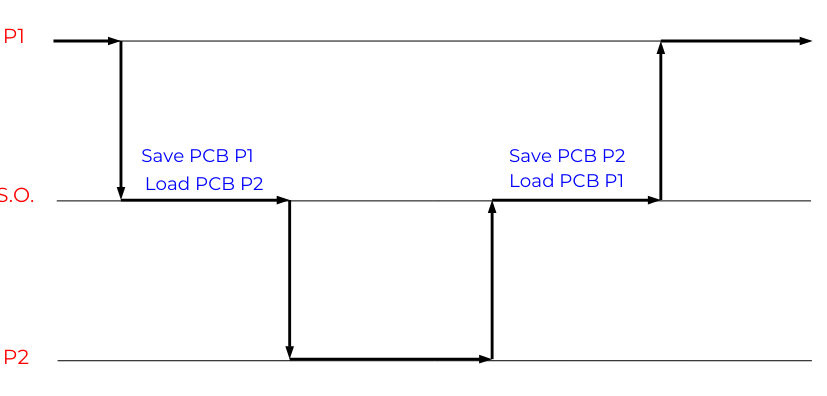
\includegraphics[width=0.7\textwidth]{img/cw.png}
\end{figure} 
\paragraph{Vita di un processo}
\begin{itemize}
  \item Running
  \item Waiting (aspetta un qualche evento esterno)
  \item Ready
\end{itemize}
Nella maggior parte dei SO i processi sono in forma gerardica padre-figli. Quello che non è specificato dal padre viene eridatato dal figlio. Ovviamente un processo può svolgere 1 sola sequenza di istruzione alla volta.\\
Nei SO però abbiamo anche i processi multithreaded ovvero sequenze di istruzioni parallele. I thread condividono dati, I/O, codice. \\
\textbf{E' conveniente?} Si, infatti creare un nuovo thread è molto più veloce che creare un nuovo processo. \\
Ma come li implementiamo?
\begin{itemize}
  \item User thread, implementati attraverso una \textit{thread library} che ci permett di non avere senza alcun intervento del kernel
  \item Kernel thread, supportati nativamenti dal kernel. Più lento perchè si passa da livello utente a livello kernel
\end{itemize}
I SO moderni li implementano tutti e due, infatti abbiamo tre differenti modelli di multithreading:
\begin{itemize}
  \item Many-to-One: un certo numero di user thread vengono mappati su un solo kernel thread
  \item One-to-One: ogni user thread viene mappato su un kernel thread
  \item Many-to-Many
\end{itemize}
\subsubsection{Scheduling}
Per rappresentare uno schedule si usano i diagrammi di Gantt
\begin{figure}[H]
    \centering
    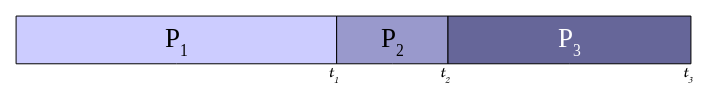
\includegraphics[width=0.7\textwidth]{img/ganttt.png}
\end{figure} 
In questo esempio da $0-t_1$ abbiamo la CPU che esegue $P_1$, e così via. \\
Nel caso di Gantt multi-risorsa lo rappresentiamo
\begin{figure}[H]
    \centering
    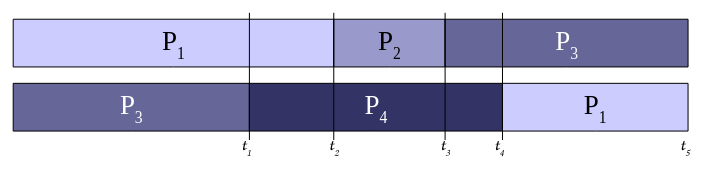
\includegraphics[width=0.6\textwidth]{img/gantt_multi.png}
\end{figure} 
Un \textbf{context switch} può avvenire a causa di
\begin{itemize}
  \item 1. Un processo passa da running a waiting 
  \item 2. Un processo passa da running a ready 
  \item 3. Un processo passa da waiting a ready
  \item 4. Un processo termina
\end{itemize}
\textit{Nota}: per $2$ e $3$ è possibile continuare ad eseguire il processo corrente.\\
\vspace{1px}
Se avvengono i context switch solo per $1$ e $4$ allora abbiamo uno scheduler \textbf{non-preemptive} (cooperativo) ovvero se il controllo della risorsa viene trasferito solo se l'assegnatario attuale lo cede volontariamente. Mentre se avviene sempre allora abbiamo uno scheduler \textbf{preemptive} ovvero è possibile che il controllo della risorsa venga tolto all'assegnatario attuale a causa di un evento (tutti gli scheduler moderni).\\
\vspace{2em}\\
Durante l'esecuzione di un processo abbiamo i momementi di attività della CPU (\textbf{CPU burst}) e i momenti di attività I/O (\textbf{I/O burst}). 
\begin{figure}[H]
    \centering
    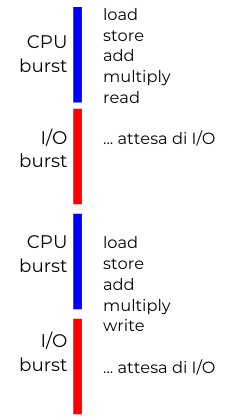
\includegraphics[width=0.15\textwidth]{img/burst.png}
\end{figure} 
Lo scheduler che algoritmo si basa?
\begin{itemize}
  \item First Come, First Served: il processo che arriva per primo, viene servito per primo (no-preemption)
  \item Shortest-Job First: la CPU viene assegnata al processo ready che ha la minima durata del CPU burst successivo (no-preemption)\\
  Sarebbe la soluzione ottimale ma è impossibile applicarla nella realtà! Possiamo solo approssimarla con due algoritmi
  \begin{itemize}
    \item Shortest-Next-CPU-Burst First (no-preemptive): il processo corrente esegue fino al completamento del suo CPU burst
    \item Shortest-Remaining-Time-First (preemptive): il processo corrente può essere messo nella coda ready, se arriva un processo con un CPU burst più breve di quanto rimane da eseguire al processo corrente
  \end{itemize}  
  \item Round-Robin: un processo non può rimanere in esecuzione per un tempo superiore alla durata del \texttt{quanto di tempo} (se breve il SO diventa inefficiente, se lungo abbiamo tanti periodi di inattività). E quindi abbiamo due possibilità:
  \begin{itemize}
    \item un processo può lasciare il processore volontariamente, in seguito ad un'operazione di I/O
    \item un processo può esaurire il suo quanto di tempo senza completare il suo CPU burst, nel qual caso viene aggiunto in fondo alla coda dei processi pronti
  \end{itemize}
  in entrambi i casi, il prossimo processo da esegure è il primo della coda dei processi pronti.
\end{itemize}
Ovviamente queste implementazioni non vanno sempre bene (es. frame video). Allora implmentiamo lo \textbf{scheduling a priorità}. \\
Ad ogni processo associamo una specifica priorità, lo scheduler sceglie il processo pronto con priorità più alta. Le priorità sono definite dal SO o dal utente. La priorità può essere statica o dinamica durante la vita di un processo. \\
\vspace{1em}\\
Possiamo ulteriormente migliorare attraverso lo \textbf{scheduling a classi di priorità} ovvero creare diverse classi di processi con caratteristiche simili e assegnare ad ogni classe specifiche priorità. La coda ready viene quindi scomposta in molteplici "sottocode", una per ogni classe di processi.\\
Per ogni classe poi possiamo pure utilizzare una politica specifica adatta alle caratteristiche della classe. Così otteniamo lo \textbf{scheduling Multilivello}.\\
\vspace{1em}\\
Possiamo anche definire lo \textbf{scheduling real-time}, ovvero la correttezza dell'esecuzione non dipende solamente dal valore del risultato, ma anche dall'istante temporale nel quale il risultato viene emesso.
\subsection{Gestione risorse e deadlock}
Le risorse le possiamo suddividere in classi. Le risorse di una classe vengono dette \textbf{istanze} della classe. Il numero di risorse in una classe viene detto \textbf{molteplicità} del tipo di risorsa.\\
Un processo non può richiedere una specifica risorsa ma solo una risorsa di una specifica classe. Come le assegniamo?
\begin{itemize}
  \item Risorse ad assegnazione statica: avviene al momento della creazione del processo e rimane valida fino alla terminazione
  \item Risorse ad assegnazione dinamica: i processi richiedono, le utilizzano e le rilasciano quando non più necessarie. (I/O)
\end{itemize}
\paragraph{Tipi di richieste}
\begin{itemize}
  \item Richiesta bloccante: il processo richiedente si sospende se non ottiene immediatamente l'assegnazione
  \item Richiesta non bloccante: la mancata assegnazione viene notificata al processo richiedente, senza provocare la sospensione
\end{itemize}
\paragraph{Tipi di risorse}
\begin{itemize}
  \item Risorse non condivisibili: una singola risorsa non può essere assegnata a più processi contemporaneamente (CPU, C.S., stampanti)
  \item Risorve condivisibili: (file aperti)
\end{itemize}
\paragraph{Risorse prerilasciabili}
Una risorsa si dice prerilasciabile (\textit{preemptable}) se la funzione di gestione può sottrarla ad un processo prima che questo l'abbia effettivamente rilasciata.\\
Il processo che subisce il prelascio si deve sospendere, la risorsa prerilasciata sarà successivamente restituita al processo.\\
La risorsa è prelasciabile se il suo stato non si modifica durante l'utilizzo (oppure il suo stato può essere facilmente salvato e ripristinato).
\paragraph{Risorse non prelasciabili}
Una risorsa si dice non prelasciabile se la funzione di gestione non può sottrarle al processo al quale sono assegnate. Sono non prerilasciabili le risorse il cui stato non può essere salvato e ripristinato.
\subsubsection{Deadlock}
Quando avviene un deadlock? Quando tutte queste condizioni devono valere tutte contemporaneamente affinché un deadlock si presenti nel sistema
\begin{itemize}
  \item Mutua esclusione: risorse non condivisibili
  \item Assenza di prerilascio: le risorse devono essere rilasciate volontariamente dai processi che le controllano
  \item Richieste bloccanti: un processo che ha già ottenuto risorse può chiederne ancora
  \item Attesa circolare: il processo $P_n$ aspetta la risorsa controllata da $P_{n+1}$ fino a $P_k$ che aspetta $P_0$.
\end{itemize}
\paragraph{Grafo di Holt}
Grafo diretto (direzione), bipartito (i nodi sono suddivisi in due sottoinsiemi \textit{<risorse, processi>} e non esistono archi che collegano nodi dello stesso sottoinsieme).
\begin{center}
  risorsa $\to$ processo := la risorsa è assegnata al processo \\
  processo $\to$ risorsa := il processo ha richiesto la risorsa
\end{center}
\begin{figure}[H]
    \centering
    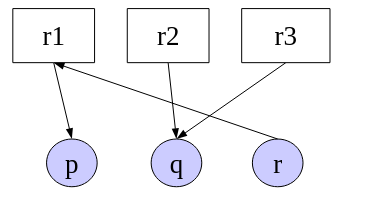
\includegraphics[width=0.3\textwidth]{img/holt.png}
\end{figure} 
\begin{itemize}
  \item Grafo di Holt in generale: l'insieme delle risorse è partizionato in classi e gli archi di richiesta sono diretti alla classe e non alla singola risorsa
  \begin{itemize}
    \item i processi sono rappresentati da \textit{cerchi}
    \item le classi sono rappresentati come \textit{contenitori rettangolari}
    \item le risorse come \textit{punti} all'interno delle classi
  \end{itemize}
  \begin{figure}[H]
    \centering
    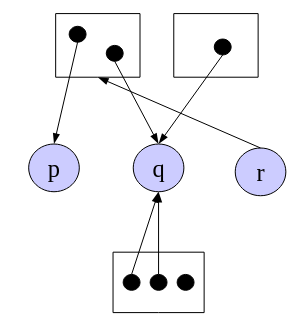
\includegraphics[width=0.3\textwidth]{img/generale.png}
\end{figure} 
  \item Grafo di Holt - Notazione operativa: grafo pesato (con pesi ai nodi risorsa e pesi sugli archi)
  \begin{itemize}
    \item Sugli archi la molteplicità di risorse o richiesta
    \item All'interno delle classi: numero di risorse non ancora assegnate
  \end{itemize}
    \begin{figure}[H]
    \centering
    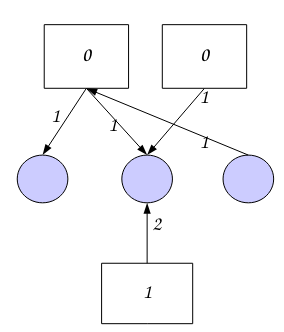
\includegraphics[width=0.3\textwidth]{img/operativa.png}
\end{figure} 
\end{itemize}
\paragraph{Metodi di gestione dei deadlock}
\begin{itemize}
  \item Deadlock detection and recovery: permettere al SO di entrare in deadlock, poi con un algoritmo lo rileviamo ed eventualmente eseguire un'azione di recovery.\\
  Mantenere aggiornato il grafo di Holt, registrando su di esso tutte le assegnazioni e le richieste di risorse. Utilizzare il grafo per rilevare gli stati di deadlock.\\
  \vspace{1em}\\
  \begin{itemize}
    \item Sistema centralizzato: \textbf{Deadlock detection con grafo di Holt}\\
     \textbf{Teorema}: se le risorse sono a richiesta bloccante, non condivisibili e non prerilasciabili, lo stato è di deadlock se e solo se il grafo di Holt contiene un ciclo
      \begin{figure}[H]
    \centering
    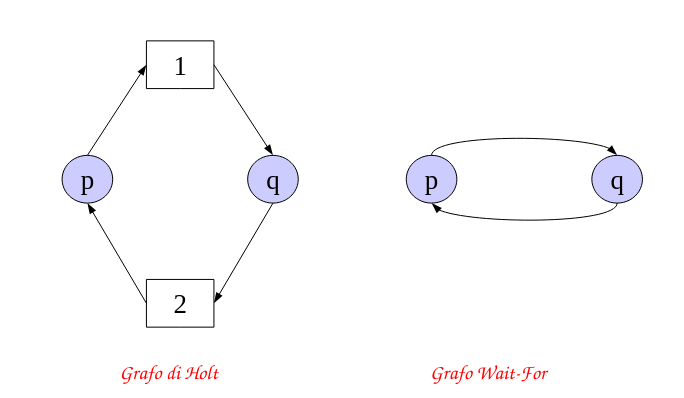
\includegraphics[width=0.6\textwidth]{img/deadlockgrafo.png}
\end{figure} 
Un grafo di Halt di può semplificare omettendo i nodi processi con solo archi entranti.\\
      \begin{figure}[H]
    \centering
    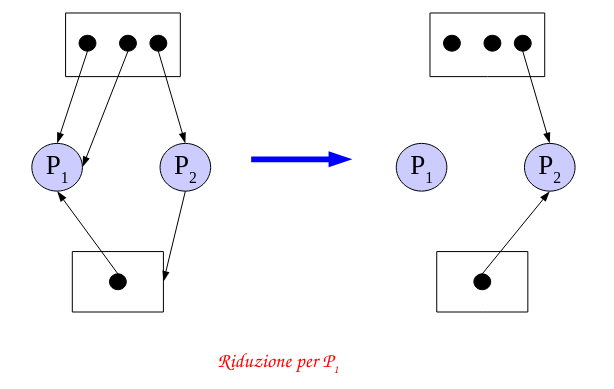
\includegraphics[width=0.5\textwidth]{img/riduzione.png}
\end{figure} 
\textbf{Teorema}: se le risorse sono a richiesta bloccante, non condivisibili e non prerilasciabili, non abbiamo deadlock se solo se il grafo di Holt è completamente riducibile.\\
    \item Sistema distribuito: \textbf{Deadlock detection - Knot} 
  \newline
  \textbf{Teorema}: Dato un grafo di Holt con una sola richiesta sospesa per processo, se le risorse sono a richiesta bloccante, non condivisibili e non prerilasciabili, allora il grafo rappresenta uno stato di deadlock se e solo se esiste un knot.
        \begin{figure}[H]
    \centering
    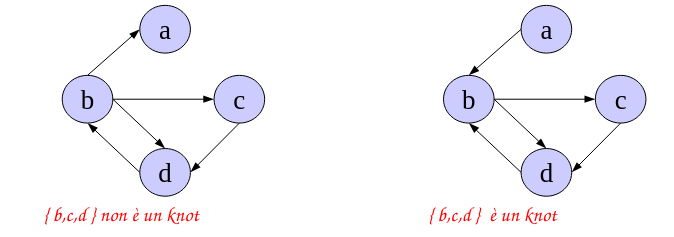
\includegraphics[width=0.6\textwidth]{img/knot.png}
\end{figure} 
\textit{Knot}: Partendo da un qualunque nodo di M ($\neq \emptyset$ t.c. $\forall n \in M \, R(n)=M$ con $R(n)$ insieme di raggiungibilità di $n$), si possono raggiungere tutti i nodi di M e nessun nodo all'infuori di esso.
  \item \textbf{Deadlock recovery} \\
  La soluzione può essere:
  \begin{itemize}
    \item \texttt{Manuale}: l'operatore viene informato e eseguirà alcune azioni che permettano al sistema di proseguire
    \item \texttt{Automatica}: il sistema operativo è dotato di meccanismi che permettono di risolvere in modo automatico la situazione, in base ad alcune politiche
    \begin{itemize}
      \item Terminazione totale: tutti i processi coinvolti vengono terminati
      \item Terminazione parziale: viene eliminato un processo alla volta, fino a quando il deadlock non scompare
      \item Checkpoint/rollback: lo stato dei processi viene periodicamente salvato su disco (\textit{checkpoint}), in caso di deadlock, si ripristina (\textit{rollback}) uno o più processi ad uno stato precedente, fino a quando il deadlock non scompare
    \end{itemize}
  
  \end{itemize}
  \end{itemize}
   \item Deadlock prevention / avoidance: impedire al sistema di entrare in uno stato di deadlock\\
    \begin{itemize}
      \item \textbf{Prevention}: Per evitare il deadlock si elimina una delle quattro condizioni del deadlock. Vediamo quale attaccare:
      \begin{itemize}
        \item \texttt{Mutua esclusione}: non è possibile, alcune risorse sono intrinsecamente non condivisibili
        \item \texttt{Richiesta bloccante}: l'\textit{allocazione totale} non è sempre possibile
        \item \texttt{Assenza di prerilascio}: non è possibile, alcune risorse sono intrinsecamente non prelasciabili. Servono interventi manuali
        \item \texttt{Attesa Circolare}: attraverso una allocazione \textit{gerardica} alle classi di risorse vengono associati valori di priorità, e i processi possono richiedere risorse solo in ordine crescente di priorità
      \end{itemize}
      \item \textbf{Avoidance}: prima di assegnare una risorsa ad un processo, si controlla se l'operazione può portare al pericolo di deadlock, se positivo l'operazione viene ritardata.\\
      \vspace{1px}\\\textit{Algoritmo del banchiere}: il banchiere deve essere in ogni istante in grado di soddisfare tutte le richieste dei clienti, o concedendo immediatamente il prestito oppure comunque facendo loro aspettare la disponibilità del denaro in un tempo finito.\\
      \vspace{1em}\\
      Defiano uno stato \textbf{SAFE} se esiste una sequenza di processi $P_1, P_2, ..., P_n$ tale che per ogni $P_i$ le risorse richieste da $P_i$ sono soddisfatte dalle risorse attualmente disponibili più le risorse detenute dai processi $P_1, P_2, \dots, P_{i-1}$. Definiamo uno stato \textbf{UNSAFE} se non è SAFE.\\
      Lo stato SAFE può essere verificato usando la sequenza che ordina in modo crescente i valori di $n_i$ (risorse ancora necessarie a $P_i$ per completare) e verificando che per ogni processo $P_i$ della sequenza, $n_{S(j)} \leq avail[j], \quad \text{ con } j=1,\dots,N$ (risorse attualmente disponibili).
    \end{itemize}
    \begin{figure}[H]
    \centering
    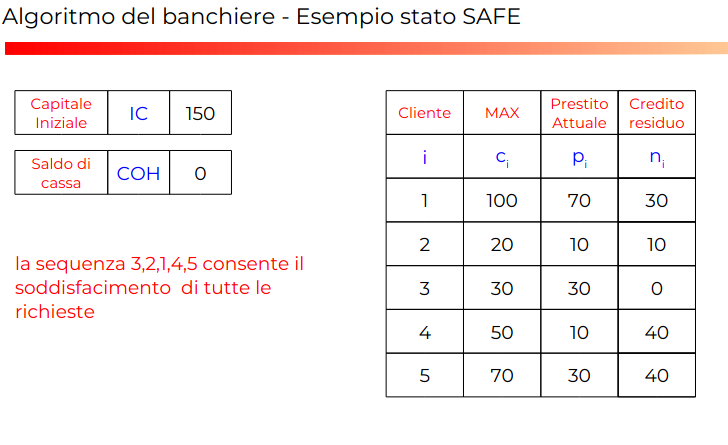
\includegraphics[width=0.7\textwidth]{img/safe.png}
\end{figure} 
\paragraph{Teorema dell'algoritmo del banchiere} Siano $C, C'$ le sequenze di processi. Sia $H = \{p \in \text{ processi } | p \notin C\}$. Sia $h$ il primo elemento di $H$ che compare in $C'$. \\
Tutti gli elementi di $C'$ prima di $h$ sono in $C$. Chiamiamo $C''$ il segmento iniziale di $C'$ fino al punto precendente l'applicazione di $h$.\\
Le risorse diponibili all'applicazione di $h$ in $C'$ sono $avail(C'')\, = \, COH + \sum_{j \in C} p_j$; $h$ e' applicabile quindi $n \leq avail(C'')$.\\
Ma $avail(C) \, = \, COH + \sum_{j \in C} p_j$ quinsi se $avail(C) \leq avail(C'')$ allora $h$ e' applicabile alla fine di $C$ contro l'ipotesi che $C$ non sia ulteriormente estendibile (SAFE).\\
   \item Ostrich algorithm (Algoritmo dello struzzo): ignorare il problema del tutto!\\
    Calcolare il costo dei deadlock puo' essere troppo elevato. (Unix, JVM)
\end{itemize}
\subsection{Gestione della memoria}
La parte del sistema operativo che gestisce la memoria principale si chiama \textbf{memory manager}. Deve tenere tarccia della memoria libera e occupata, allocare memoria ai processi e deallocarla quando non serve piu'.
\subsubsection{Binding, loading, linking}
Con il termine binding si indica l'associazione di indirizzi logici di memoria (e.g. nomi di variabili, label) ai corrispodenti indirizzi fisici. Questa avviene a:
\begin{itemize}
  \item \textbf{Tempo di compilazione}: gli indirizzi vengono calcolati al momento della compilazione e resteranno gli stessi ad ogni esecuzione del programma. Non e' compatibile con la multiprogrammazione.
  \begin{figure}[H]
    \centering
    
\includegraphics[width=0.7\textwidth]{img/compilazione.png}
\end{figure} 
Questo e' leggero, semplice e non richiede hw speciale.
  \item \textbf{Tempo di caricamento}: il codice generato dal compilatore non contiene indirizzi assoluti ma relativi
    \begin{figure}[H]
    \centering
    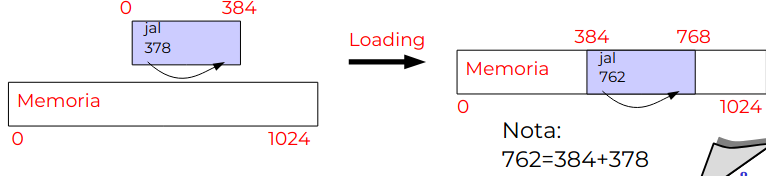
\includegraphics[width=0.7\textwidth]{img/caricamento.png}
\end{figure} 
Funziona in multiprogrammazione, non serve hw speciale ma richiede una traduzione degli indirizzi da parte del loader, e quindi formati particolare dei file eseguibili.
  \item \textbf{Tempo di esecuzione}: l'individuazione dell'indirizzo di memoria effettivo viene effettuata durante l'esecuzione da un componente hardware apposito: la memory management unit (MMU)
    \begin{figure}[H]
    \centering
    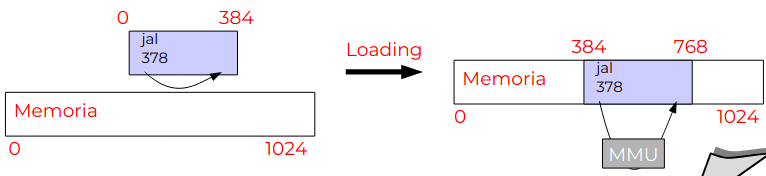
\includegraphics[width=0.7\textwidth]{img/esecuzione.png}
\end{figure} 
\end{itemize}
\paragraph{Prestazioni speciali}
\begin{itemize}
  \item \texttt{Loading dinamico}: caricare alcune routine di libreria solo quando vengono richiamate (ddl). Tutte le routine a caricamento dinamico risiedono su un disco (codice rilocabile), quando servono vengono caricate, dipende dal programmatore quali e come utilizzarle.
  \item \texttt{Linking dinamico}: E' possibile posticipare il linking delle routine di libreria al momento del primo riferimento durante l'esecuzione, ovvero collegare le librerie in fase di esecuzione invece che durante la compilazione. Consente di avere eseguibili più compatti.
\end{itemize}
\subsubsection{Allocazione contigua}
\begin{itemize}
  \item \textbf{Allocazione contigua}: tutto lo spazio assegnato ad un processo deve essere formato da celle consecutive. 
  \item \textbf{Allocazione non contigua}: è possibile assegnare a un processo aree di memorie separate
  \item \textbf{Allocazione statica}: un processo deve mantenere la propria aerea di memoria dal  caricamento alla terminazione
  \item \textbf{Allocazione dinamica}: durante l'esecuzione, un processo può essere spostato all'interno della memoria
\end{itemize}
Ora vediamo diverse tipologie di allocazione:
\begin{itemize}
  \item \texttt{Allocazione a partizioni fisse} (contigua-statica): è possibile utilizzare una coda per partizione, oppure una coda comune per tutte le partizioni. Va bene per SO monoprogrammati (MS-DOS, sistemi embedded)
      \begin{figure}[H]
    \centering
    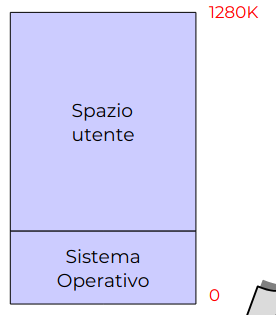
\includegraphics[width=0.2\textwidth]{img/fisse.png}
\end{figure} 
  \item \texttt{Frammentazione interna}: se un processo occupa una dimensione inferiore a quella della partizione che lo contiene, lo spazio non utilizzato è sprecato. La presenza di spazio inutilizzato all'interno di un'unità di allocazione si chiama \textbf{frammentazione interna}.
      \begin{figure}[H]
    \centering
    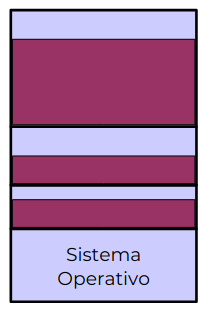
\includegraphics[width=0.2\textwidth]{img/interna.png}
\end{figure} 
  \item \texttt{Allocazione a partizioni dinamiche} (contigua-statica): la memoria disponibile (nella quantità richiesta) viene assegnata ai processi che ne fanno richiesta
      \begin{figure}[H]
    \centering
    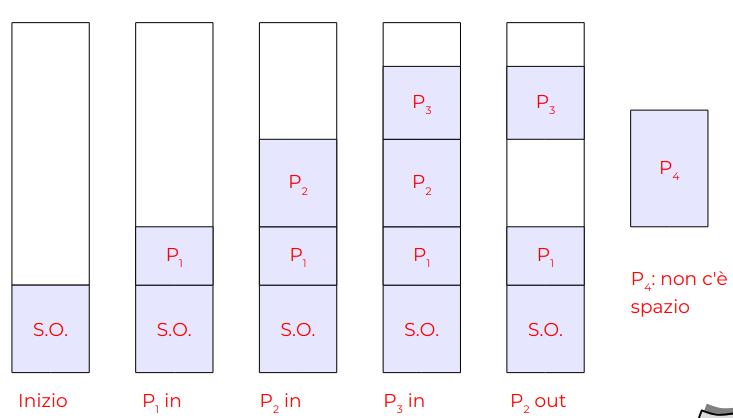
\includegraphics[width=0.7\textwidth]{img/dinamica.png}
\end{figure} 
  \item \texttt{Frammentazione esterna}: dopo un certo numero di allocazioni e deallocazioni di memoria dovute all'attivazione e alla terminazione dei processi lo spazio libero appare suddiviso in piccole aree, il fenomeno è detto \textbf{frammentazione esterna}.
  \item \texttt{Compattazione}: se è possibile rilocare i processi durante la loro esecuzione, è allora possibile procedere alla \textbf{compattazione} della memoria. Risolve il problema della frammentazione esterna.
      \begin{figure}[H]
    \centering
    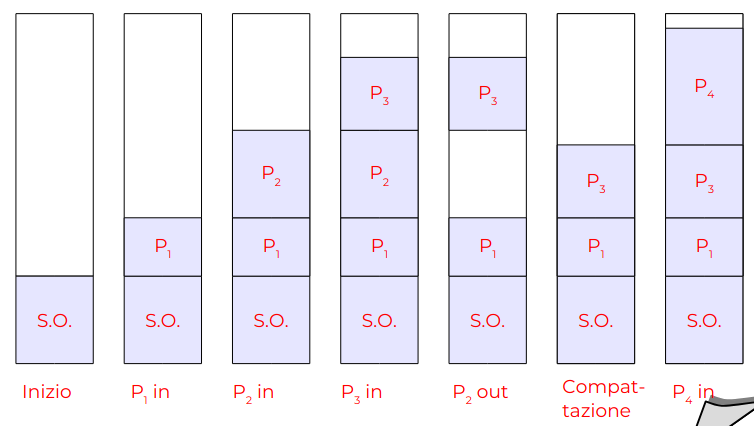
\includegraphics[width=0.7\textwidth]{img/compattazione.png}
\end{figure} 
  \item Strutture di dati (dinamica):
  \begin{itemize}
    \item Mappa di bit: memoria suddivisa in blocchi, per ogni blocco un bit per indicare se occupata (1) o no (0).
          \begin{figure}[H]
    \centering
    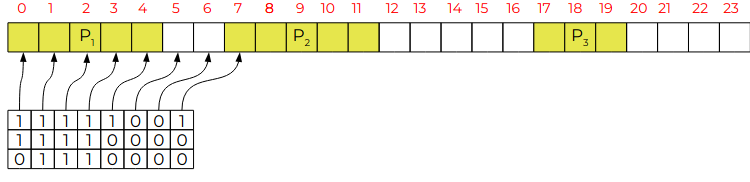
\includegraphics[width=0.7\textwidth]{img/bit.png}
\end{figure} 
    Il costo per trovare un insieme di blocchi contigui liberi e' $O(n)$.
    \item Lista con puntatori: una lista che segna per ogni $L$ se e' occupata $P$ o libera $H$, viene segnata anche la dimensione del blocco \textit{<inizio, fine>}. 
              \begin{figure}[H]
    \centering
    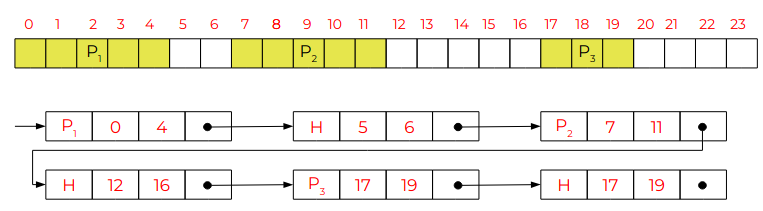
\includegraphics[width=0.7\textwidth]{img/lista.png}
\end{figure} 
    Per allocare un processo di dimensione $n$ si scorre la lista fino a trovare un blocco libero di dimensione $m \geq n$. Poi la vecchia lista $H$ diventa $P \to H'$, con $H'$ di dimensione $m-n$ blocchi. Costo: $O(n)$\\
    Per deallocare, se abbiamo altri $H$ vicini si crea un unico blocco libero accorpandoli. Costo: $O(1)$.
    \end{itemize}
\end{itemize}
Nella allocazione dinamica come scegliare il blocco libero?
\begin{itemize}
  \item \texttt{First fit}\phantomsection\label{first_fit}: si scorre la lista dei blocchi liberi e si assegna il primo blocco di dimensione $m \geq n$ trovato
  \item \texttt{Next fit}: come First Fit, ma invece di ripartire sempre dall'inizio, parte dal punto dove si era fermato all'ultima allocazione. Evita frammentazione all'inizio della memoria, ma non è molto efficiente se la memoria è molto frammentata. Ha performance peggiori rispetto a First Fit.
  \item \texttt{Best fit}: si scorre tutta la lista dei blocchi liberi e si assegna il blocco di dimensione $m \geq n$ più piccolo possibile. Riduce la frammentazione esterna, ma è più lento di First Fit.
  \item \texttt{Worst fit}: eleziona il più grande fra i blocchi liberi presenti in memoria. Riduce la frammentazione esterna, ma è più lento di First Fit.
\end{itemize}
\subsubsection{Paginazione}
\label{paginazione}
Approccio moderno per ridurre la frammentazione interna ed elimina quella esterna. Pero' serve hw speciale (MMU).
\begin{figure}[H]
    \centering
    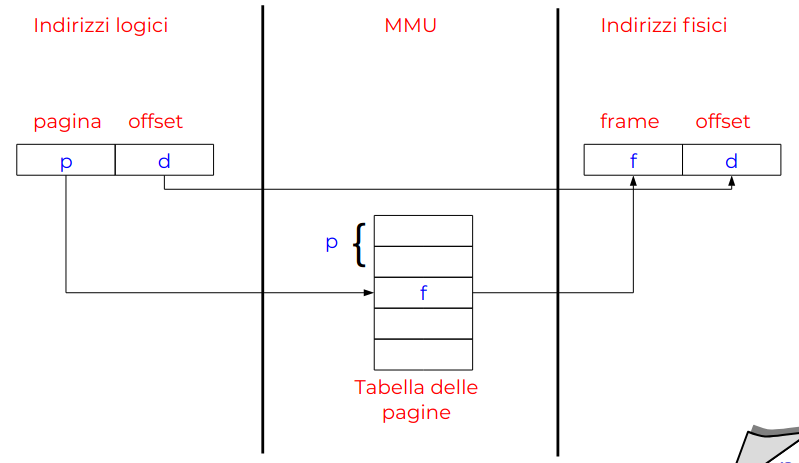
\includegraphics[width=0.7\textwidth]{img/MMU.png}
\end{figure} 
\begin{itemize}
  \item La memoria fisica e' divisa in \textbf{frame}, ovvero blocchi di dimensione fissa. Deve essere una potenza di 2, tipicamente 4KB.\\
  Pagine troppo piccole portano a una tabella grande, mentre pagine troppo grandi portano a frammentazione interna.
  \item La memoria logica e' divisa in \textbf{pagine} della stessa dimensione dei frame.
  \item Quando un processo chiede memoria, si allocano un numero sufficienti di frame (anche non contigui).
\end{itemize}
\begin{figure}[H]
    \centering
    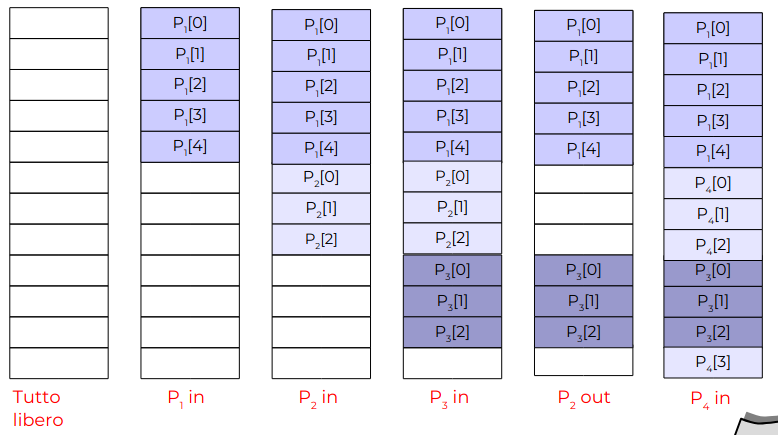
\includegraphics[width=0.7\textwidth]{img/frame.png}
\end{figure} 
\begin{figure}[H]
    \centering
    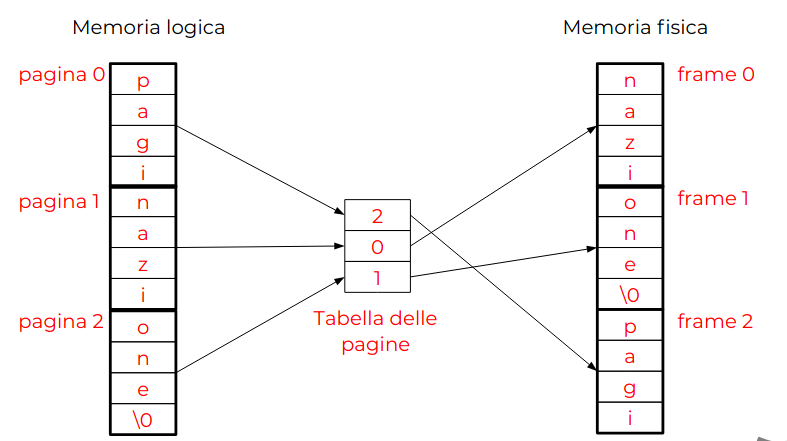
\includegraphics[width=0.7\textwidth]{img/frame2.png}
\end{figure} 
Dove metiamo la tabella delle pagine?
\begin{itemize}
  \item Registri dedicati: un insieme di registri all'interno del MMU. Questo pero' e' troppo costoso.
  \item Memoria: il numero di accessi in memoria pero' raddoppia, prima alla tabella e poi al dato.
  \item Translation lookaside buffer (\textbf{TLB}): insieme di registri (solo 8-2048 registri) suddivisi in due parti \textit{<chiave, valore>}. Per cercare un dato cerchiamo la sua chiave e se presente (\textit{TLB hit}) si ritorna il valore; in caso contario (\textit{TLB miss}) si accede alla tabella in memoria e si ritorna il valore. 
\begin{figure}[H]
    \centering
    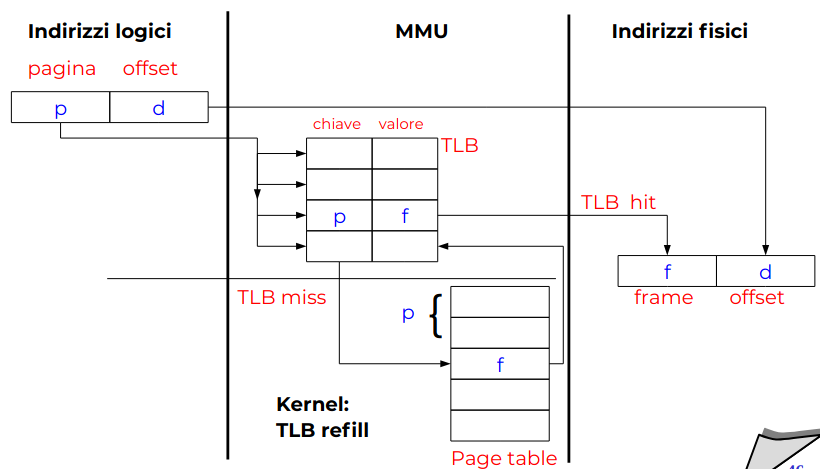
\includegraphics[width=0.7\textwidth]{img/tlb.png}
\end{figure} 
  Ovviamente questo modello di cache come tutti si basa sul principio di localita'.
\end{itemize}
\subsubsection{Segmentazione}
In un sistema a segmentazione la memoria di un processo e' suddivisa in aree differenti. Quindi lo spazio di indirizzamento logico e' dato da un insieme di segmenti (aree di memoria continua con \textit{<nome segmento, lunghezza>}). Questo pero' spett al programmatore/compilatore la suddivisione dei programmi in segmenti. \\
\paragraph{Segmentazione e condivisione?} E' possibile condividere un segmento tra più processi, ad esempio il segmento di codice di una libreria condivisa o la comunicazione fra i processi. 
\begin{figure}[H]
    \centering
    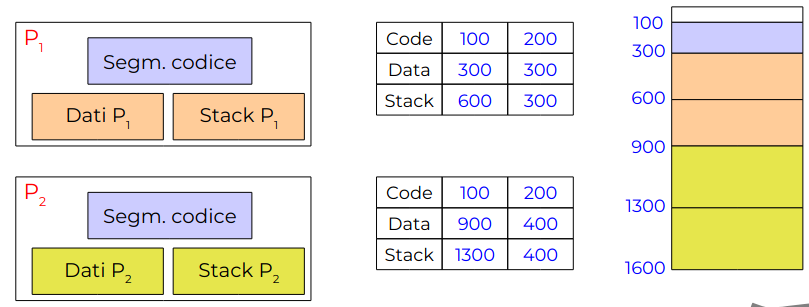
\includegraphics[width=0.7\textwidth]{img/condivisione.png}
\end{figure} 
Il problema della segmentazione e' che se abbiamo segmenti di \textbf{dimensione variabile} allora soffriamo di frammentazione esterna, mentre se abbiamo segmenti di \textbf{dimensione fissa} allora soffriamo di frammentazione interna. Potremmo teoricamente utilizzare tecniche di allcazione dinamica come \hyperref[first_fit]{First Fit}. Ma abbiamo gli stessi problemi di frammentazione della allocazione dinamica.\\
\paragraph{Segmentazione + paginazione} E se combinassimo le due tecniche? Ogni segmento viene suddiviso in pagine che vengono allocate in frame liberi della memoria (non necessariamente contigui).\\
A livello hw dobbiamo avere una MMU che supporti sia la segmentazione che la paginazione.\\
Cosi avremo pero' sia i benefici della segmentazione (protezione, condivisione) che quelli della paginazione (no frammentazione esterna).
\subsubsection{Memoria virtuale}
E' la tecnica che permette l'esecuzione di processi che non sono completamente in memoria.\\
Questo permette di eseguire processi che richiedono più memoria di quella fisica disponibile. A contro pero' se implementata male, la memoria virtuale, puo' rallentare un sistema.
\paragraph{Non infrange i requisiti di un'architettura di Von Neumann?} No, perche' l'architettura di Von Neumann dice che le istruzioni da eseguire e i dati su cui operano devono essere in memoria, ma non e' detto che l'intero spazio di indirizzamento logico sia in memoria o sia utilizzato del tutto.
\paragraph{Implementazione della memoria virtuale} Ogni processo ha uno spazio di \textit{indirizzamento virtuale} (anche piu' grande di quello fisico se serve). Gli indirizzi logici virtuali posso essere mappati su indirizzi fisici della memoria principale oppure su memoria secondaria.\\
In caso di accesso a dati su memoria secondaria i dati vengono trasferiti su memoria principale o se fosse piena si sposta in memoria secondaria i dati contenuti in memoria principale che sono considerati meno utili (swap).\\
\vspace{1em}\\
\subsubsection*{Demand paging}
La \textbf{paginazione a richiesta }utilizza la tecnica di \hyperref[paginazione]{paginazione} ammettendo però che alcune pagine possano essere in memoria secondaria.\\
Ci segnamo nelle tabella delle pagina se una pagina e' in memoria principale o secondaria, attarverso un bit $v$ (\textit{valid bit}).\\
\vspace{1px} \textbf{Cosa succede se accediamo a una pagina che non e' in memoria?} Il processore genera un trap \hyperref[page_fault]{\textbf{page fault}} e il \hyperref[pager]{\textbf{pager}} (componente del SO) si occupa di caricare la pagian mancante e di aggiornare la tabella delle pagine.
\begin{figure}[H]
    \centering
    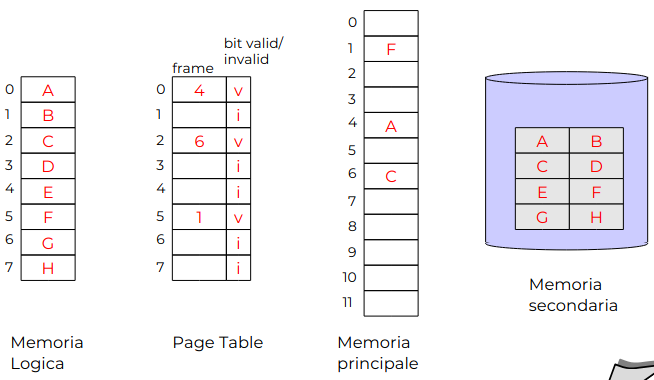
\includegraphics[width=0.7\textwidth]{img/memvrt.png}
\end{figure} 
\subsubsection*{Pager}\label{pager}
Il pager (in passato \textbf{swapper}) si occupa di gestire la \textbf{swap area} (l'area del disco utilizzata per ospitare le pagine in memoria secondaria).\\
\begin{itemize}
  \item In passato avevamo lo \textbf{swap} ovvero copiare l'intera area are di memoria di in processo da mem. principale alla secondaria (\textit{swap-in}) o l'inverso (\textit{swap-out}).
  \item Potremmo anche utilizzare una tecnica di \textbf{paginazione su richiesta}, ovvero carichiamo solo quello che serve. Potrebbe funzionare ma e' una tecnica di \textit{lazy swap}.
\end{itemize}
\subsubsection*{Gestione dei page fault}\label{page_fault}
In caso di mancanza di frame liberi che facciamo? Dobbiamo liberare il frame "\textit{meno utile}".\\
Possiamo utilizzare un \texttt{algoritmo di rimpiazzamento}, ovvero minimizzare il numero di page fault.  \\
\vspace{1px}\\
\textbf{Algoritmo del meccanismo di demand paging}:
  \begin{itemize}
    \item Individua la pagina di memoria secondaria'
    \item Individua un frame libero
    \item Se il frame libero non esiste
    \begin{itemize}
      \item richiamo algoritmo di rimpiazzamento
      \item aggiorna tabella delle pagfine
      \item se la pagina "vittima" era stata modificata, aggiorniamola sul disco
      \item aggiorna tabella dei frame segnando che abbiamo il frame libero
    \end{itemize}
    \item Aggiorna la tabella dei frame segnando che ora quel frame e' occupato
    \item Leggiamo la pagina richiesta
    \item Aggiorniamo la tabella delle pagine
    \item Riattiva il processo
\end{itemize}
\textbf{Algoritmo di rimpiazzamento}
\begin{itemize}
  \item Algoritmo FIFO: quando dobbiamo liberare un frame liberiamo il primo frame che e' stato caricato in memoria. Questo non richiede hw specifico, e' veloce ma alcune volte scarta pagine utilizzate. \\
  Provoca un effetto dove $+\text{pagine} \Rightarrow +\text{page fault}$
  \item Algoritmo MIN - Ottimale: algoritmo teorico che seleziona come pagina vittima una pagina che non sarà più acceduta o la pagina che verrà acceduta nel futuro più lontano
  \item Algoritmo LRU (Least Recently Used): seleziona come pagina vittima la pagina che è stata usata meno recentemente nel passato.\\
  Per implementarla serve hw specifico, la MMU deve registrare nella tabella delle pagine un time-stamp quando accede ad una pagina, il time-stamp può essere implementato come un contatore che viene incrementato ad ogni accesso in memoria.\\
  \vspace{1px}\\
  Puo' essere implementata via uno stack (LIFO) di pagine, nel quale che tutte le volte che una pagina viene acceduta, viene rimossa dallo stack (se presente) e posta in cima allo stack stesso.
  \vspace{1px}\\
  \textbf{Teorema: un algoritmo a stack non genera casi di \hyperref[Belady]{anomalia di Belady}}. Se consideri l’insieme delle pagine in memoria per un dato numero di frame, questo insieme è sempre un sottoinsieme dell’insieme delle pagine che avresti con un numero maggiore di frame.
  \begin{align*}
    S_t(s,A,m) \subseteq S_t(s,A,m+1)
  \end{align*}
  con $S_t(s,A,m)$ insieme della pagine mantenute al tempo $t$ dell'algoritmo $A$, data una memoria di $m$ frame relativamente alla stringa $s$.\\
  \vspace{2px}\\
  L'algoritmo \textit{LRU} e' a stack. Vediamo come implementarlo:\\
  pagina 87
\end{itemize}
Definiamo l'\textbf{anomalia di Belady}\phantomsection\label{Belady}: quando all'aumentare delle pagine aumentano i page fault, come per l'algoritmo FIFO.\\
Non e' sempre detto che all'aumentare delle pagine aumentino i page fault come in FIFO. Dipende tutto dal algortimo scelto. Infatti per \textit{Algoritmo MIN - Ottimale} o per \textit{LRU} all'aumentare delle pagine diminuiscono i page fault. 
\begin{figure}[H]
    \centering
    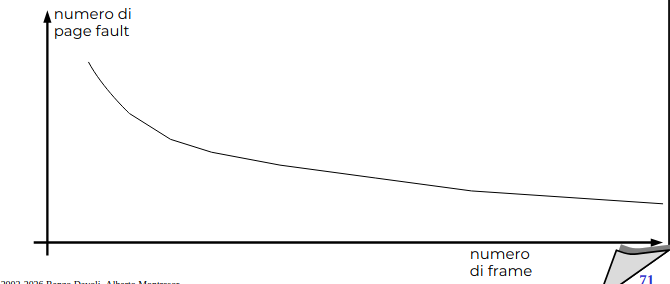
\includegraphics[width=0.7\textwidth]{img/Belady.png}
\end{figure} 
\subsection{Gestione I/O, Memoria secondaria}
\begin{figure}[H]
    \centering
    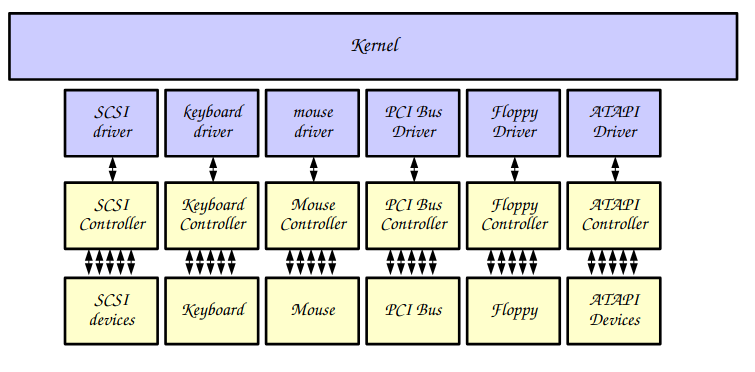
\includegraphics[width=0.7\textwidth]{img/io.png}
\end{figure} 
Come classifichiamo un sistema I/O? La modalita' di trasferimento puo' essere a \textbf{blocchi o caratteri}.\\
\begin{itemize}
  \item Blocchi: I dati vengonoi scritti/letti a blocchi (512byte), tramite filesystem e memory-mapped I/O (contenuto di un file viene mappato in memoria).
  \item Caratteri: I dati vengono letti/scritti un carattere alla volta, bufferizzazione di una linea alla volta.
\end{itemize}
\subsubsection{Progettazione del sistema di I/O}
\begin{itemize}
  \item Buffering: per gestire una differenza di velocità tra il produttore e il consumatore di un certo flusso di dati, gestire la differenza di dimensioni nell'unità di trasferimento
  \item Caching: mantiene una copia in memoria primaria di informazioni che si trovano in memoria secondaria (nel buffer troviamo una istanza della informazione, qua una copia!)
  \item Spooling: buffer che mantiene output per un dispositivo che non può accettare flussi di dati distinti (es. stampanti)
  \item I/O scheduling
\end{itemize}
\begin{figure}[H]
    \centering
    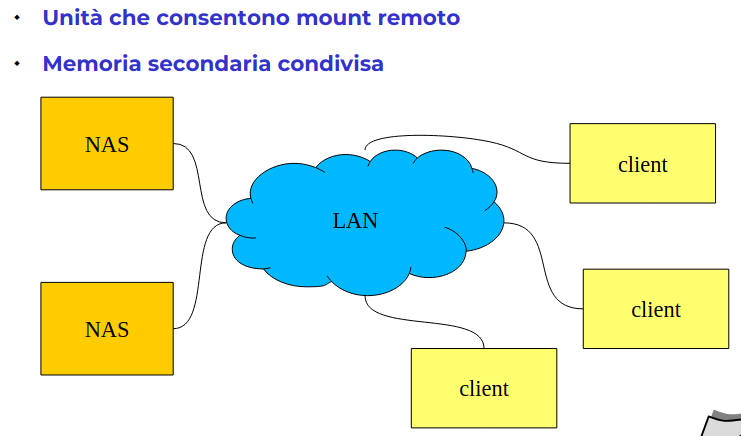
\includegraphics[width=0.7\textwidth]{img/nas.png}
\end{figure} 
\begin{figure}[H]
    \centering
    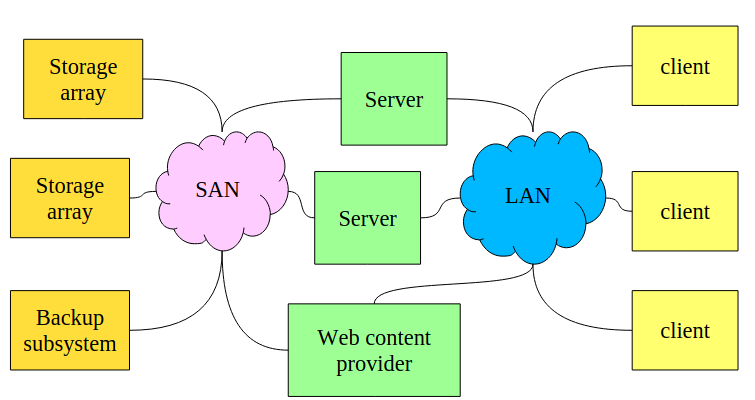
\includegraphics[width=0.7\textwidth]{img/san.png}
\end{figure} 
\subsubsection{Memoria Secondaria}
\paragraph{SSD} Gli SSD (Solid State Disk) consumano meno energia dei HDD, non hanno fragilita' meccanica, hanno un ciclo massimo di scritture. Si leggi a blocchi e si legge a \textbf{banchi} (molti blocchi), questo porta $V_\text{lettura} >> V_\text{scrittura}$ e un accesso uniforme a tutto lo spazio di memoria.
\paragraph{Dischi} Un disco è composto da un insieme di piatti, suddivisi in tracce, le quali sono suddivise in settori.
\begin{itemize}
  \item $r$ velocita' di rotazione in $rpm$, 5400/7200/10k rpm
  \item $T_s$ tempo di seek (tempo medio necessario affinchè la testina si sposti sulla traccia desiderata), circa 8-10ms
  \item $V_r$ velocità di trasferimento, espressa in byte al secondo
\end{itemize}
Caratteristiche dei dischi:
\begin{itemize}
  \item Il \textit{tempo di accesso} e' il tempo necessario per leggere un settore del disco, questo si calcola con tempo di seek + ritardo rotazionale e tempo di trasferimento.\\
  \item Il \textit{Ritardo rotazionale} e' il tempo medio necessario affinchè il settore desiderato arrivi sotto la testina, ovvero $\frac{1}{2r}$
  \item Il \textit{Transfer time}: dipende dalla quantita' dei dati $b$ de leggere, ovvero $\frac{b}{V}$
\end{itemize}
Nel SO troviamo il \textbf{gestione software dei dischi}, ovvero per rendere piu' efficiente le richieste pendenti utilizziamo un ordine che minimizza le operazioni che richiedono molto tempo (seek). Vediamone alcuni:
\begin{itemize}
  \item FCFS (First Come, First Served)/FIFO: non minimizza il numero di seek, non genera starvation
  \begin{figure}[H]
    \centering
    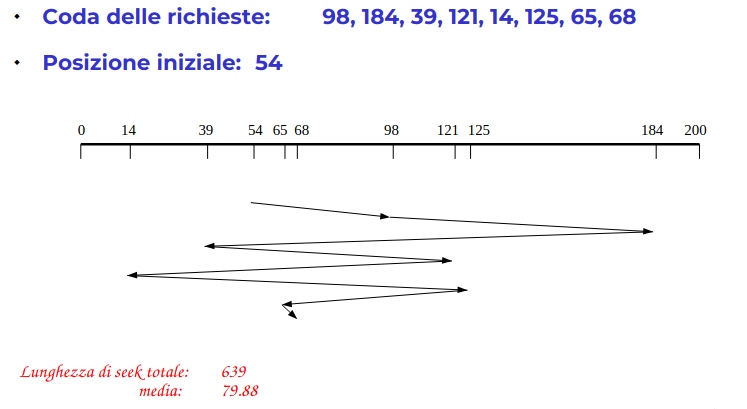
\includegraphics[width=0.7\textwidth]{img/fcfs.png}
\end{figure} 
  \item SSTF (Shortest Seek Time First): seleziona la richieste che prevede il minor spostamento della testina dalla posizione corrente, puo' provocare starvation
  \begin{figure}[H]
    \centering
    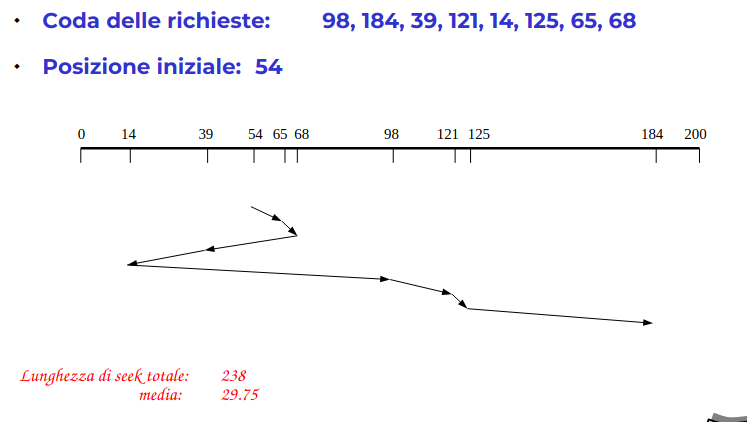
\includegraphics[width=0.7\textwidth]{img/sstf.png}
\end{figure} 
  \item LOOK (algoritmo dell'ascensore): efficente, privilegia le tracce centrali, non ha starvation
  \begin{itemize}
    \item ad ogni istante, la testina è associata ad una direzione
    \item la testina si sposta di richiesta in richiesta, seguendo la direzione scelta
    \item quando si raggiunge l'ultima richiesta nella direzione scelta, la direzione viene invertita e si eseguono le richieste nella direzione opposta
  \end{itemize}
    \begin{figure}[H]
    \centering
    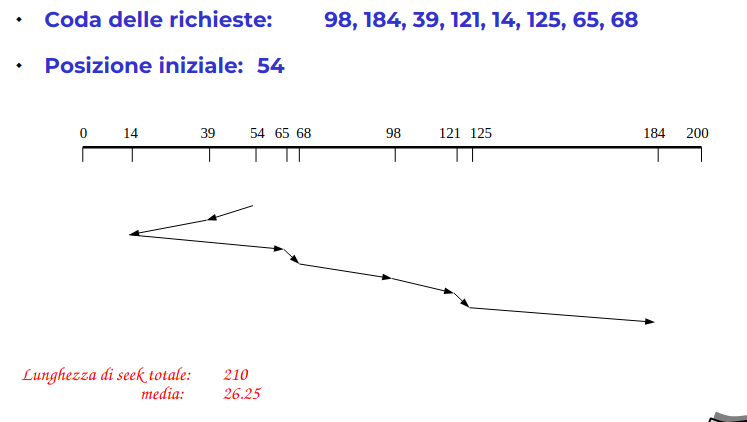
\includegraphics[width=0.7\textwidth]{img/look.png}
\end{figure} 
  \item C-LOOK: stesso principio di funzionamento del metodo LOOK, ma la scansione del disco avviene in una sola direzione
  \begin{itemize}
    \item quando si raggiunge l'ultima richiesta in una direzione, la testina si sposta direttamente alla prima richiesta
      \begin{figure}[H]
    \centering
    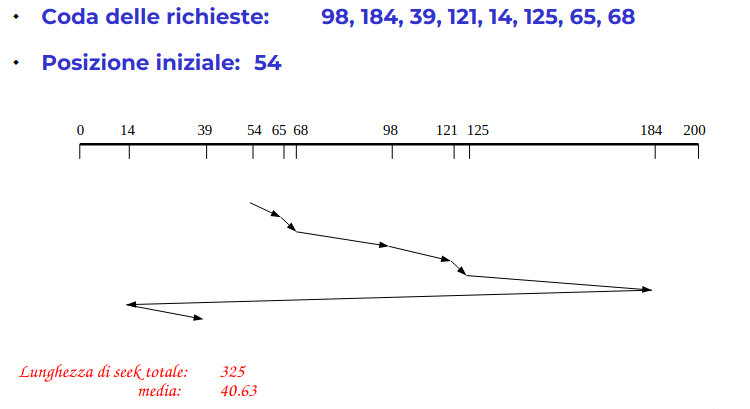
\includegraphics[width=0.7\textwidth]{img/clook.png}
\end{figure} 
  \end{itemize}
\end{itemize}
\textit{Nota}: sia per LOOK e C-LOOK è possibile che il braccio della testina non si muova per un periodo considerevole di tempo. Per risolvere:
\begin{itemize}
  \item la coda delle richieste può essere suddivisa in due sottocode separate
  \item mentre il disk scheduler sta soddisfacendo le richieste di una coda, le richieste che arrivano vengono inserite nell'altra
  \item quando tutte le richieste della prima coda sono state esaurite, si scambiano le due code
\end{itemize}
\subsubsection{RAID}
La velocità dei processori cresce secondo la legge di Moore, la velocità dei dispositivi di memoria secondaria molto più lentamente. Come risolviamo? \\
Per aumentare la velocità di un componente, una delle possibilità è quella di utilizzare il parallelismo!\\
Utilizzare un \textbf{array di dischi} indipendenti, che possano gestire più richieste di I/O in parallelo.\\
\vspace{1px}\\
Il RAID (Redundant Array of Independent Disks) consiste in 7 schemi diversi he rappresentano diverse architetture di distribuzione dei dati.\\
La capacità ridondante dei dischi può essere utilizzata per memorizzare informazioni di parità, che garantiscono il recovery dei dati in caso di guasti.\\
\vspace{1px}\\
Il SO deve presentare al disco richieste che possano essere soddisfatte in modo efficiente per ottimizzare per performance, tipo richieste di lettura di grandi quantità di dati sequenziali.
\paragraph{RAID 0 (striping)} Non possiede meccanismi di ridondanza, i dati vengono distribuiti su più dischi. Se abbiamo richiesti su due blocchi indipendenti c'e' la possibilita' che siano su dischi differenti e quindi le due richieste possono essere servite in parallelo.  \\
Il sistema RAID viene visto come un disco logico, i dati nel disco logico vengono suddivisi in strip (multiplo di settori/blocchi). Strip consecutivi sono distribuiti su dischi diversi, aumentando le performance della lettura dei dati sequenziali.
      \begin{figure}[H]
    \centering
    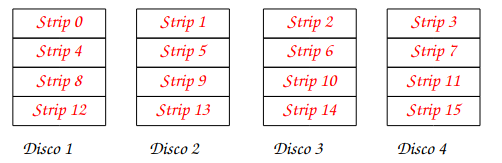
\includegraphics[width=0.7\textwidth]{img/raid0.png}
\end{figure} 
\paragraph{RAID 1 (mirroring)} La ridondanza è ottenuto duplicando tutti i dati su due insiemi indipendenti di dischi, basato su triping ma questa volta uno strip viene scritto su due dischi diversi
      \begin{figure}[H]
    \centering
    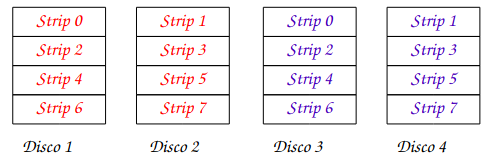
\includegraphics[width=0.7\textwidth]{img/raid1.png}
\end{figure} 
Una richiesta di lettura può essere servita da uno qualsiasi dei dischi che ospitano il dato, può essere scelto quello con tempo di seek minore.\\
Una richiesta di scrittura deve essere servita da tutti i dischi che ospitano il dato, dipende dal disco con tempo di seek maggiore.
\paragraph{RAID 4} Si utilizza il meccanismo di data striping, con strip relativamente grandi. Strip di parità calcolato a partire dagli strip di dati corrispondenti, calcolato bit-per-bit. Lo strip di parità viene posto sul disco di parità.
      \begin{figure}[H]
    \centering
    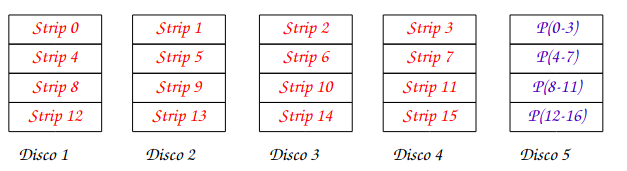
\includegraphics[width=0.7\textwidth]{img/raid4.png}
\end{figure} 
\paragraph{RAID 5} Rispetto al RAID4 abbiamo il vantaggio è che non esiste un disco di parità che diventa un bottleneck
      \begin{figure}[H]
    \centering
    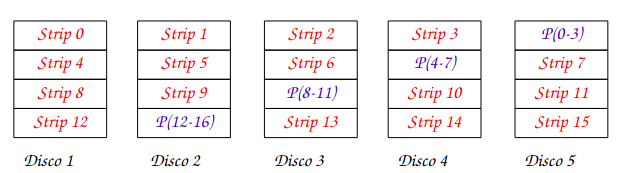
\includegraphics[width=0.7\textwidth]{img/raid5.png}
\end{figure} 
\paragraph{RAID 6} Come RAID 5, ma si utilizzano due strip di parità invece di uno. Questo aumenta l'affidabilita'.
\subsection{}
















\pagebreak
\section{Linguaggio C per Sistemi Operativi}
Il linguaggio C è un linguaggio di programmazione imperativo, strutturato e compilato, nato negli anni '70 per lo sviluppo di sistemi operativi, in particolare UNIX. \\
Il Kernel e' un componente obbligatorio dei SO moderni, vediamo di cosa gestice:
\begin{itemize}
  \item Esegue le funzioni di sistema critiche e interagisce con l’hardware (gestione CPU, memoria per i processi, fs, dispositivi, ecc)
  \item Caricato in memoria durante il boot e rimane sempre in memoria fisica
\end{itemize}
Ovviamente questo non basta per definire un SO, percio dobbiamo avere anche altre utiity
\begin{itemize}
  \item Programmi
  \item Librerie
  \item System call (per comunicare con il Kernel)
  \item Una \textit{shell} (interprete dei comandi in exec/fork) per gestire I/O e pipeline.
\end{itemize}
\subsection{Unix}
Uniplexed Information and Computing Service nasce fra gli anni '60 e '70 come sistema operativo proprietario
\begin{itemize}
  \item multiutente
  \item multitasking
  \item portatite (essendo scritto in C poteva girare su piu macchine)
  \item minimale
  \item TCP/IP (dal 1984) permise di comunicare fra piu macchine diverse
\end{itemize}
Negli anni, il codice sorgente di UNIX è stato concesso in licenza a varie università e aziende. Ognuna ha creato una propria “versione” di Unix, adattata alle proprie esigenze hardware o commerciali (Solaris di Oracle, BSD Unix, ecc). Ad oggi solo i sistemi certificati (come MacOS) sotto il marchio registrato di The Open Group possono definirsi, legalmente, Unix.
\begin{figure}[H]
    \centering
    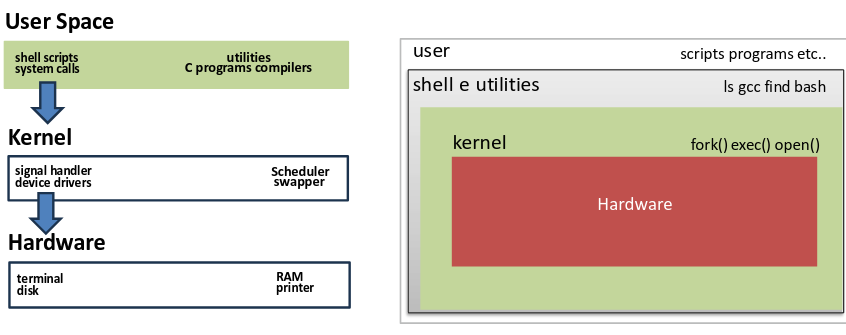
\includegraphics[width=0.7\textwidth]{img/kernel_layout.png}
\end{figure} 
Ad oggi troviamo molti \textit{Unix-like}, ovvero SO che si basano su vecchi ceppi di Unix o si ispirano fortemente
\begin{itemize} 
  \item BSD: FreeBSD, OpenBDS, NetBSD (non sono certificati come Unix ma derivano storicamente da Unix)
  \item MacOS / IOS (basati su BSD + kernel XNU) \\
  XNU = "X is not Unix" e' un kernel sviluppato da Apple ibrido, ovvero BSD + March (processi, trhead, memoria, ecc) + Driver (proprietari)
  \item Linux: Linux e’ un kernel libero compatibile con Unix distribuito con licenza GPL, partendo da zero, cioè senza usare alcuna riga di codice Unix. Si basa sugli strumenti GNU. Si occupa di gestire: \\
  - Processi \\
  - Memoria \\
  - Driver \\
  - Filesystem \\
  - Networking 
\end{itemize}
Tutti 3 gli OS qui sopra si basano sullo standard POSIX (Portable Operating System Interface, with an X for Unix), è una famiglia di standard sviluppata dall’IEEE a partire dagli anni ’80 (serie IEEE 1003), in collaborazione con ISO. Uno standard del genere ci permette di avere software portatili tra i sistemi operativi Unix-like, attraverso API, comandi e comportamenti comuni.
\subsection{Cosa definisce POSIX?}
\begin{itemize}
  \item System call, API: per la gestione dei processi come "fork(), exec(), wait(), ecc", gestione dei file "open(), read(), write(), gestione della IPC per pipe, semafori, memoria condivisa, "kill(), signal()"
  \item Comandi di base: "ls, cp, mv, ecc"
  \item Shell
\end{itemize}
\subsection{GNU}
l progetto GNU (Richard Stallman, Free Software Foundation, dal 1983) voleva creare un sistema operativo libero in stile Unix.
GNU sviluppo': librerie (glibc), compilatore (gcc), shell (bash), strumenti base. Mancava ancosa pero' un kernel! Si e' fatta una prova con "GNU Hub" ma si decise di andare con il kernel linux. Definiamo \textbf{GNU/Linux} il sistema operativo completo. \\
Ovviamente essendo un modello libero, Unix-like con standard POSIX e molto flessibile in breve tempo si diffusero diverse \texttt{distribuzioni}.
\begin{figure}[h] % [h] = qui (here)
    \centering
    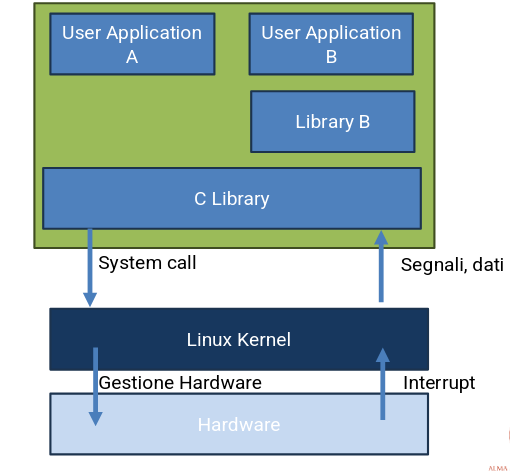
\includegraphics[width=0.3\textwidth]{img/linux_kernel.png}
\end{figure} \\
Il kernel deve occuparsi delle risorse hw (CPU, memoria, IO), deve fornire delle API portatili e standarizzate tra le architetture, gestire accessi concorrenti. \\
Fra lo \textit{user space} e il kernel troviamo le system call, ovvero un set di comandi del kernel (circa 400 ad oggi). Tutte le system call le troviamo nella libreria C, ma non le chiamiamo mai direttamente ma convochiamo le rispettive versione della funzione in C. \\
Il filesystem segue convenzioni come FHS (filesystem hierarchy standard)
\begin{itemize}
  \item / (root), /bin, /usr, /lib, /etc, /dev, /proc, /sys.
  \item /dev (dispositivi come file speciali)
  \item /proc, /sys (informazioni del kernel e device in modo file-like)
\end{itemize}
\vspace{2em}
Il C rimane essenziale dove contano controllo e prevedibilità: \\
- kernel, driver, librerie di base, sistemi embedded ed edge. \\
- Senza garbage collector e con puntatori espliciti, rende chiari i rapporti tra sicurezza e prestazioni.\\
Quindi possiamo definire il C come il linguaggio privilegiato quando servono efficienza, interoperabilità e un legame diretto con l’hardware.
\end{document}
